\documentclass[11pt,letterpaper]{article}

\usepackage[margin=1in]{geometry}
\usepackage[T1]{fontenc}
\usepackage[utf8]{inputenc}
\usepackage{lmodern}
\usepackage{microtype}
\usepackage{amsmath,amssymb,mathtools,bm,mathrsfs}
\usepackage{booktabs,tabularx,array}
\usepackage{xcolor}
\usepackage[most]{tcolorbox}
\usepackage{enumitem}
\usepackage{fancyhdr}
\usepackage{tikz}
\usetikzlibrary{calc, arrows.meta, positioning, fit, backgrounds, shapes.geometric,
                decorations.markings}
\usepackage[hidelinks]{hyperref}

\definecolor{deepblue}{RGB}{25,55,90}
\definecolor{softblue}{RGB}{236,244,250}
\definecolor{softgreen}{RGB}{237,247,239}
\definecolor{softorange}{RGB}{252,244,231}
\definecolor{softgray}{RGB}{244,244,244}
\definecolor{deepgreen}{RGB}{30,90,45}

\hypersetup{
  pdftitle={Gauge-Covariant Variational Free Energy: A Physicist's Companion},
  pdfauthor={MultiAgentELBO project},
  pdfsubject={Principal bundles, associated law bundles, variational free energy, holonomy, and effective scale theory}
}

\pagestyle{fancy}
\fancyhf{}
\lhead{\textit{Gauge-covariant variational free energy}}
\rhead{\textit{Physicist's companion}}
\cfoot{\thepage}
\setlength{\headheight}{14pt}

\setlength{\parindent}{0pt}
\setlength{\parskip}{0.7em}
\setlist[itemize]{leftmargin=1.6em,itemsep=0.25em,topsep=0.25em}

\newcommand{\KL}{\operatorname{KL}}
\newcommand{\Prob}{\mathbb P}
\newcommand{\Rec}{\mathbb Q}
\newcommand{\Post}{\boldsymbol\Pi}
\newcommand{\Law}{\mathcal P}
\newcommand{\id}{\operatorname{id}}
\newcommand{\ev}{\operatorname{ev}}
\newcommand{\Ad}{\operatorname{Ad}}
\newcommand{\Tr}{\operatorname{Tr}}
\newcommand{\GL}{\mathrm{GL}}
\newcommand{\Ex}{\mathbb E}

\newtcolorbox{physicalreading}{
  colback=softblue,
  colframe=deepblue,
  title=Physical reading,
  fonttitle=\bfseries,
  breakable
}

\newtcolorbox{provedbox}{
  colback=softgreen,
  colframe=green!45!black,
  title=What is established,
  fonttitle=\bfseries,
  breakable
}

\newtcolorbox{boundarybox}{
  colback=softorange,
  colframe=orange!65!black,
  title=Boundary of the result,
  fonttitle=\bfseries,
  breakable
}

\newtcolorbox{translationbox}{
  colback=softgray,
  colframe=black!55,
  title=Translation,
  fonttitle=\bfseries,
  breakable
}

\newtcolorbox{proposalbox}{
  colback=softgreen,
  colframe=deepgreen,
  title=Proposed extension beyond the current main manuscript,
  fonttitle=\bfseries,
  breakable
}

\title{\textbf{Gauge-Covariant Variational Free Energy}\\[0.35em]
\Large A Physicist's Companion to the Full Theory}
\author{MultiAgentELBO theory program}
\date{August 16, 2026}

\begin{document}

\maketitle

\begin{abstract}
This document is an orientation to the full gauge-covariant variational free energy manuscript, written for a reader who knows gauge theory, statistical mechanics, and the renormalization group, and who does not want to begin with measure-theoretic disintegration. The theory is a genuine gauge theory whose matter fields are probability laws rather than vectors: one principal bundle over a contextual base, two associated bundles carrying belief and model laws in possibly inequivalent representations, chosen connections with their transports and holonomies, and an exact variational identity with the dimensionless Helmholtz form of an expected energy minus an entropy. Multi-agent attention is a canonical Gibbs ensemble on each source simplex, with a row free energy that must retain its entropy term. A normalized attention weight is not a chemical potential; a genuine grand-canonical extension requires a separate fluctuating edge or membership count. Coarse graining is a normalized Markov channel, the information it discards is measured exactly, and a pointwise meta-agent exists only after the channel pushes the full generative, recognition, and posterior laws. Throughout, the emphasis falls on which statements are theorems in the main manuscript, which are modeling declarations, which are thermodynamic analogies, and which are proposed extensions.
\end{abstract}

\tableofcontents
\newpage

\section{What this document is}

The technical manuscript is a long, deliberately austere development. Every nontrivial sentence in it carries a status tag, hypotheses are never suppressed for readability, and constructions that a physicist would ordinarily perform in one line are separated into a declaration, a theorem, and a boundary statement. That discipline is the point of the manuscript, but it makes for slow reading, and it can obscure the fact that the underlying picture is a familiar one.

The picture is this. Take a gauge theory. Replace the matter fields, which ordinarily take values in a vector space carrying a representation of the structure group, by probability laws, on which the group acts by pushforward. Give the theory an action principle, not by postulating a Lagrangian, but by importing the exact variational identity that relates log evidence, a variational bound, and a relative entropy. Then ask the renormalization question: which of this structure survives when microscopic degrees of freedom are replaced by effective ones, and how much information is destroyed in the replacement.

What follows summarizes that program at the level of detail a graduate physicist would want from a colloquium and a careful conversation afterward. It states the main results, gives the physical analogies that make them recognizable, and is explicit about the places where the analogy is exact, the places where it is suggestive only, and the places where the manuscript itself declines to make a claim.

Two companion documents already exist. The technical source is the manuscript assembled from \path{Theory/main.tex}, and a separate guide, \path{solid_RG_theory.tex}, treats the static pointwise coarse-graining theorem in depth. This document is wider and shallower than either. Where a compact statement here appears to differ from a technical qualification there, the manuscript controls.

\section{The theory in one paragraph}

Fix a smooth manifold \(\mathcal C\) of contexts and a principal \(G\)-bundle \(\mathscr P_G\to\mathcal C\). Two associated bundles \(\mathcal E_b\) and \(\mathcal E_m\) carry, in their fibers, spaces of probability laws: beliefs about a latent state, and laws over model presentations. An agent is a local section of both, together with its choice of local frame. Because different agents may choose different frames, their laws cannot be compared until transported, and transport around a closed loop returns a possibly nontrivial group element, the holonomy. On a finite design the theory declares one normalized generative joint law over observations and latents and one correlated recognition law, and the exact identity
\begin{equation}
  \log p_\theta(o\mid X)
  =\mathcal L(\Rec_X;X)
  +\KL\bigl(\Rec_X\Vert\Prob_\theta(\cdot\mid o,X)\bigr)
  \label{eq:elbo-identity}
\end{equation}
splits the log evidence into a variational bound and a nonnegative gap. For many agents, one collective free energy governs everything, and each exact local update is a coordinate move on it. Entropy-regularized source selection is a canonical ensemble whose energies depend on transported disagreement, so beliefs and effective bonds can coevolve without yet producing a meta-agent. A pointwise parent is constructed only when one normalized recognition-independent channel pushes the complete fine generative, recognition, and posterior laws. That pushforward preserves the evidence and gives an exact conditional-information defect. Turning a sequence of such parent constructions into a renormalization group requires additional identifications between changing state spaces, while turning adaptive source weights into a grand-canonical topology requires separate count-bearing occupation variables. The multivariate Gaussian appears only at the end, as an optional computational realization in which the abstract objects become matrix formulas.

\begin{physicalreading}
The main manuscript supplies variational flows on spaces of probability laws at a fixed context, and it supplies typed arrows between scales. It does not identify either construction with physical time, derive an autonomous field theory on the base, or prove sustained nonequilibrium. A free-energy descent, a trajectory semiconjugacy, a scale diagram, and a physical dynamics are four different statements.
\end{physicalreading}

\section{A physicist's dictionary}

\begin{table}[ht]
\centering
\small
\begin{tabularx}{\textwidth}{>{\raggedright\arraybackslash}p{0.235\textwidth}X}
\toprule
\textbf{Object in the theory} & \textbf{Nearest familiar object} \\
\midrule
\(\mathscr P_G\to\mathcal C\) & A principal gauge bundle, exactly as in Yang--Mills. The base is not spacetime. \\
\(\mathcal E_b,\mathcal E_m\) & Two matter sectors in possibly inequivalent representations of one group, as quarks and gluons carry the fundamental and adjoint. Here the fibers are spaces of probability laws. \\
\(\rho_b,\rho_m\) & The two representations. \(\widehat\rho\) denotes the induced action on laws, by pushforward, not by multiplying a density. \\
\(u_i^b,u_i^m\) & Two choices of local gauge, not two bundles. \\
\(h_i\) with \(u_i^m=u_i^b h_i\) & The group-valued field comparing the two gauge choices. \\
\(A_i=(u_i)^*\omega\) & The gauge potential in a local frame, with the usual \(\Ad_{a^{-1}}A+a^{-1}da\) law. \\
\(\Omega_\gamma,\widetilde\Omega_\gamma\) & Wilson lines: path-ordered transport of the two matter sectors. \\
\(\Theta_e\in G\) & A lattice link variable on the declared interaction graph. \\
\(H(\gamma)=\prod_a\Theta_{e_a}\) & A Wilson loop. Its conjugacy class is gauge invariant. \\
\(\Phi,\widetilde\Phi\) & Declared maps between the two matter sectors. Extra structure, not forced by the gauge group. \\
\(\mathcal D\Phi\) & The covariant defect: the failure of a cross-sector map to commute with transport. \\
\(\log p_\theta(o\mid X)\) & A log normalizer or log partition function. Its negative is the minimum of the dimensionless variational functional at the selected record. \\
\(\mathcal L(\Rec)\) & The Gibbs--Bogoliubov--Feynman variational bound. \\
\(\KL(\Rec\Vert\Post)\) & The exact gap of that bound. \\
\(\mathcal F=-\mathcal L\) & Variational free energy. \\
\(H_o(y)=-\log L_o(y)\) & The interaction energy of a configuration given the record. \\
\(\mathcal F_i^{\mathrm{row}}\) & A canonical Helmholtz free energy on the source simplex: expected mismatch plus temperature times relative entropy to the source prior. \\
\(\beta_{ij}\) & A conditional source-occupation probability. It is neither inverse temperature nor a chemical potential; \(\tau_i\) is the row temperature. \\
\(\rho_{ij},\mu_{ij}\) & In the proposed grand-canonical extension, an edge-occupation probability and its conjugate chemical potential. These variables are not part of the established main theorem. \\
\(C_A(dz\mid y)\) & A block-spin rule, allowed to be stochastic. \\
\((\Prob_A,\Rec_A,\Post_A)\) & The full pointwise parent probabilistic datum obtained by pushing all three fine laws through the same channel. A pair of pooled marginals is not a substitute. \\
\(\Delta_A\) & The information the block spin erases, computed exactly. \\
\(g^F\) & The Fisher metric, equal to the Hessian of the exponential-family log partition function; a susceptibility. \\
\(h_s^\omega\) & The Fisher metric pulled back to the base along a section, using a chosen connection. \\
\((L,\Lambda)\) & Interaction and total precision. Only the generalized eigenvalues of the pencil are frame independent. \\
\bottomrule
\end{tabularx}
\caption{A translation between the manuscript's objects and standard physics vocabulary. The right column is an orientation aid; each row is qualified in the section that treats it.}
\label{tab:dictionary}
\end{table}

\section{The gauge structure}

\subsection{The base is not spacetime}
\label{sec:base}

The base \(\mathcal C\) is a finite-dimensional smooth, second countable, Hausdorff manifold whose points are called contexts. It is declared, and the declaration proves nothing. What matters is the list of things it is not. It is not the population index set \(V=\{1,\dots,N\}\) of agents, and it is not their interaction graph. It is not a latent sample space. It is not physical spacetime, and the manuscript supplies no Lorentzian signature, no causal cones, no measure on \(\mathcal C\), and no field equation for it.

What the base does supply is a smooth structure supporting curves and differential forms, so that a connection on a bundle over \(\mathcal C\) defines transport along curves in \(\mathcal C\). It does not thereby define parallel transport of tangent vectors of \(\mathcal C\) itself, since \(\mathscr P_G\) has not been identified with the frame bundle. The finite design \(D=\{c_a\}\) used in the probability chapters is a finite subset of \(\mathcal C\), not a discretization theorem and not a sample from a law on \(\mathcal C\); no expectation over contexts is ever taken.

The base is also fixed and timeless. A curve in \(\mathcal C\) orders contexts; it does not by itself represent an agent evolving. Belief change at a fixed context is a curve inside one associated fiber, and simultaneous change over all contexts is a curve in a declared space of sections. These are different constructions and the manuscript keeps them apart.

\begin{boundarybox}
A physicist reading ``base manifold with a connection'' will want to put a metric on \(\mathcal C\), write an action, and vary it. The manuscript does not do this and does not claim it can be done. The only geometry the base receives is a pullback semimetric that is relative to a chosen connection and a chosen section, and that can be degenerate. No canonical connection is selected anywhere in the manuscript.
\end{boundarybox}

\subsection{One principal bundle, two matter representations}

The ambient geometry is one principal right \(G\)-bundle \(\pi:\mathscr P_G\to\mathcal C\), together with two associated bundles
\begin{equation}
  \mathcal E_b=\mathscr P_G\times_{\widehat\rho_b}\mathcal B_b,
  \qquad
  \mathcal E_m=\mathscr P_G\times_{\widehat\rho_m}\mathcal B_m,
  \label{eq:associated}
\end{equation}
where \(\mathcal B_b\subseteq\Law(\mathsf K)\) and \(\mathcal B_m\subseteq\Law(\mathsf M)\) are declared spaces of normalized probability laws. The representations \(\rho_b\) and \(\rho_m\) need not be equivalent, faithful, or of equal dimension. This is the ordinary situation in a gauge theory with several matter sectors: one group, several representations, several fiber dimensions. Figure~\ref{fig:bundle} shows the arrangement.

\begin{figure}[ht]
\centering
\resizebox{\textwidth}{!}{%
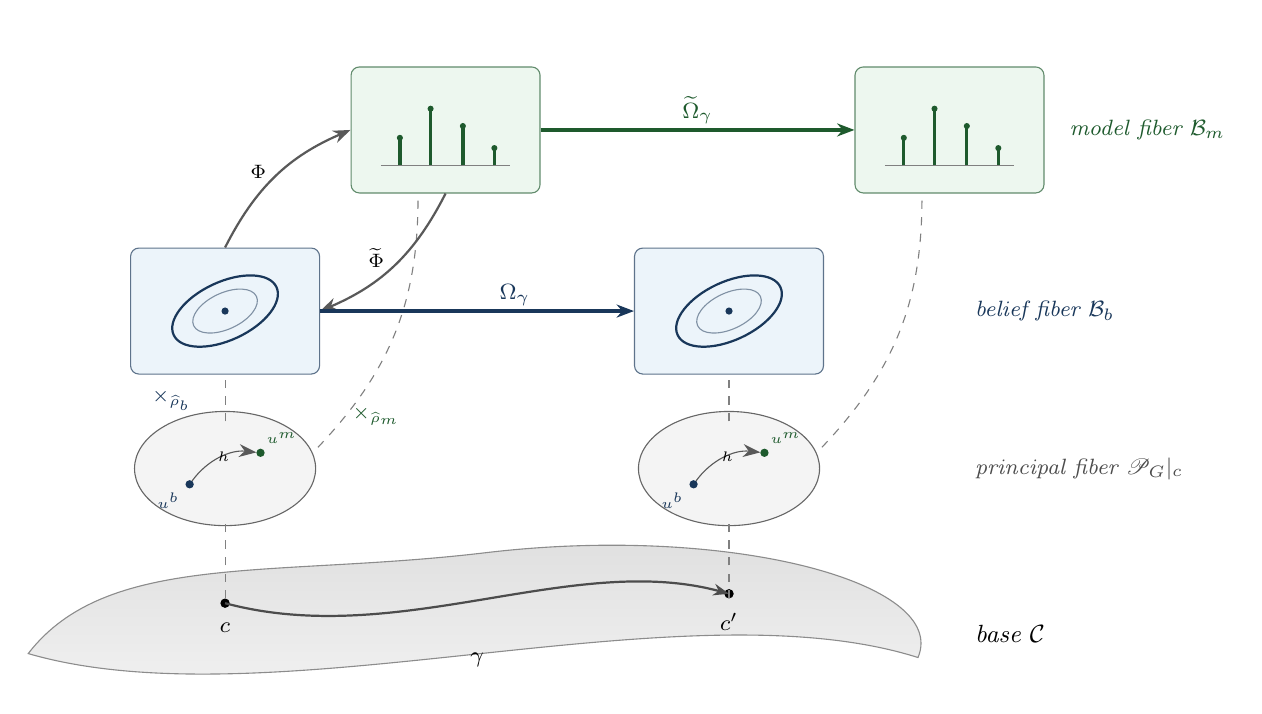
\begin{tikzpicture}[
  >={Stealth[length=2.2mm]},
  every node/.style={font=\small},
  bfib/.style={draw=deepblue!70, fill=softblue, rounded corners=3pt,
               minimum width=2.4cm, minimum height=1.6cm},
  mfib/.style={draw=deepgreen!70, fill=softgreen, rounded corners=3pt,
               minimum width=2.4cm, minimum height=1.6cm},
  pfib/.style={draw=black!60, fill=softgray, ellipse,
               minimum width=2.3cm, minimum height=1.45cm},
  assoc/.style={dashed, black!50}
]
\shade[top color=black!13, bottom color=black!4, draw=black!45]
  (-0.7,-0.6) .. controls (2.4,-1.5) and (7.6,0.3) .. (10.6,-0.65)
  .. controls (11.0,0.3) and (8.2,1.05) .. (5.1,0.68)
  .. controls (2.4,0.36) and (0.3,0.7) .. (-0.7,-0.6) -- cycle;
\node[anchor=west, font=\small\itshape] at (11.2,-0.35) {base $\mathcal C$};
\fill (1.8,0.04) circle (1.7pt) node[below=1.3mm, font=\footnotesize] {$c$};
\fill (8.2,0.16) circle (1.7pt) node[below=1.3mm, font=\footnotesize] {$c'$};
\draw[thick, black!70, -{Stealth[length=2mm]}]
  (1.8,0.04) .. controls (4.0,-0.55) and (6.2,0.7) .. (8.2,0.16);
\node[font=\footnotesize] at (5.0,-0.68) {$\gamma$};
\node[pfib] (P1) at (1.8,1.75) {};
\node[pfib] (P2) at (8.2,1.75) {};
\foreach \x in {1.8, 8.2}{
  \draw[assoc] (\x,0.10) -- (\x,1.15);
  \fill[deepblue]  (\x-0.45,1.55) circle (1.5pt);
  \fill[deepgreen] (\x+0.45,1.95) circle (1.5pt);
  \draw[->, black!65, shorten >=1.5pt, shorten <=1.5pt]
    (\x-0.45,1.55) to[bend left=30] (\x+0.45,1.95);
  \node[font=\tiny, text=deepblue]  at (\x-0.72,1.34) {$u^b$};
  \node[font=\tiny, text=deepgreen] at (\x+0.72,2.14) {$u^m$};
  \node[font=\tiny] at (\x-0.02,1.90) {$h$};
}
\node[anchor=west, font=\footnotesize\itshape, text=black!70] at (11.2,1.75)
  {principal fiber $\mathscr P_G|_c$};
\node[bfib] (B1) at (1.8,3.75) {};
\node[bfib] (B2) at (8.2,3.75) {};
\foreach \cx in {1.8, 8.2}{
  \draw[assoc] (\cx,2.35) -- (\cx,2.95);
  \begin{scope}[shift={(\cx,3.75)}]
    \draw[deepblue, thick, rotate=25] (0,0) ellipse (0.72 and 0.37);
    \draw[deepblue!55, rotate=25] (0,0) ellipse (0.44 and 0.23);
    \fill[deepblue] (0,0) circle (1.3pt);
  \end{scope}
}
\node[font=\scriptsize, text=deepblue] at (1.12,2.62) {$\times_{\widehat\rho_b}$};
\node[anchor=west, font=\footnotesize\itshape, text=deepblue] at (11.2,3.75)
  {belief fiber $\mathcal B_b$};
\node[mfib] (M1) at (4.6,6.05) {};
\node[mfib] (M2) at (11.0,6.05) {};
\foreach \cx in {4.6, 11.0}{
  \begin{scope}[shift={(\cx,6.05)}]
    \draw[black!50] (-0.82,-0.45) -- (0.82,-0.45);
    \foreach \p/\hh in {-0.58/0.35, -0.19/0.72, 0.22/0.5, 0.62/0.22}{
      \draw[deepgreen, very thick] (\p,-0.45) -- (\p,-0.45+\hh);
      \fill[deepgreen] (\p,-0.45+\hh) circle (1.1pt);
    }
  \end{scope}
}
\draw[assoc] (2.98,2.02) to[bend right=22] (4.25,5.25);
\draw[assoc] (9.38,2.02) to[bend right=22] (10.65,5.25);
\node[font=\scriptsize, text=deepgreen] at (3.72,2.42) {$\times_{\widehat\rho_m}$};
\node[anchor=west, font=\footnotesize\itshape, text=deepgreen] at (12.4,6.05)
  {model fiber $\mathcal B_m$};
\draw[->, thick, black!65] (B1.north) to[bend left=20] (M1.west);
\node[font=\scriptsize] at (2.22,5.52) {$\Phi$};
\draw[->, thick, black!65] (M1.south) to[bend left=20] (B1.east);
\node[font=\scriptsize] at (3.72,4.42) {$\widetilde\Phi$};
\draw[->, very thick, deepblue] (B1.east) --
  node[above, font=\footnotesize, fill=white, inner sep=1.5pt, pos=0.62]{$\Omega_\gamma$} (B2.west);
\draw[->, very thick, deepgreen] (M1.east) --
  node[above, font=\footnotesize, fill=white, inner sep=1.5pt, pos=0.5]{$\widetilde\Omega_\gamma$} (M2.west);
\end{tikzpicture}}
\caption{\textbf{The ambient geometry.} One principal bundle over the contextual base carries two associated bundles whose fibers are spaces of probability laws: a belief fiber, drawn as a covariance ellipse, and a model fiber, drawn as a law over model presentations. Each agent chooses two local frames \(u^b\) and \(u^m\) in the same principal fiber, related by the group-valued field \(h\). Separate connections transport the two sectors along a base curve. The cross maps \(\Phi\) and \(\widetilde\Phi\) are declared extra structure; they are not principal-bundle morphisms and are not assumed to be inverses.}
\label{fig:bundle}
\end{figure}

Two points in this arrangement are easy to get wrong, and the manuscript spends real effort on both.

The first concerns what the gauge group is. Independently rechoosing the two local trivializations,
\begin{equation}
  u_i^{b\prime}=u_i^b a_i,
  \qquad
  u_i^{m\prime}=u_i^m b_i,
  \label{eq:reframing}
\end{equation}
is a passive change of coordinates with two independent parameters, and it is tempting to read it as a \(G\times G\) gauge symmetry. It is not. The principal gauge group is the single group of \(G\)-equivariant automorphisms of \(\mathscr P_G\) covering the identity, and each such automorphism acts on both associated bundles at once. Writing the local functions of one automorphism \(F\) as \(F(u_i^b)=u_i^b k_i^b\) and \(F(u_i^m)=u_i^m k_i^m\), equivariance forces
\begin{equation}
  k_i^m=h_i^{-1}k_i^b h_i,
  \label{eq:diagonal-gauge}
\end{equation}
so the two local descriptions of one gauge transformation are conjugate, not independent. A product gauge theory with two genuinely independent principal bundles is available as an optional extension, but it carries extra topology and should be invoked only when those degrees of freedom are actually wanted.

The second concerns the group action. The action on laws is the pushforward,
\begin{equation}
  \widehat\rho_b(g)q=(\rho_b(g))_{\#}q,
  \qquad\text{so}\qquad
  \bigl(\widehat\rho_b(g)q\bigr)(A)=q\bigl(\rho_b(g)^{-1}A\bigr),
  \label{eq:pushforward-action}
\end{equation}
and this is not the same as multiplying a matrix into a density. For a Gaussian belief with mean \(\mu\) and covariance \(\Sigma\), and \(R=\rho_b(g)\) linear and invertible, the pushforward is the congruence
\begin{equation}
  \mu\mapsto R\mu,
  \qquad
  \Sigma\mapsto R\Sigma R^\top,
  \qquad
  J=\Sigma^{-1}\mapsto R^{-\top}JR^{-1},
  \label{eq:congruence}
\end{equation}
which is the transformation law a physicist would expect for a covariant two-tensor and its inverse. Much of the Gaussian part of the manuscript is bookkeeping about this congruence.

\subsection{Fibers of laws, and what that costs}

Replacing a vector fiber by a fiber of probability laws is the one structural novelty, and it has consequences that a reader trained on vector bundles should anticipate.

A law fiber carries no linear structure, so there is no covariant derivative in the usual sense on a merely measurable law fiber, and no curvature two-form acting on it by matrix multiplication. Differential statements are made only on a declared smooth tier, where the law fibers are finite-dimensional smooth parametrized-measure models closed under the group action and the action is smooth. Even there, the Fisher tensor is a Riemannian metric only when it is nondegenerate, and it is called a semimetric until nondegeneracy is proved.

A law fiber is also not a kernel fiber. A point of \(\mathcal B_m\) is a law over model presentations, a single presentation is a sample, and the generative mechanism that presentation denotes is a Markov kernel obtained by an evaluation map. These are three different types, and the manuscript is emphatic that conflating them is the commonest error in the model sector. The evaluation map is not assumed injective, so distinct presentations may denote the same mechanism, and no regularity is claimed for the quotient.

Finally, the cross maps \(\Phi:\mathcal E_b\to\mathcal E_m\) and \(\widetilde\Phi:\mathcal E_m\to\mathcal E_b\) are declared data. Sharing a structure group does not produce a map between the two associated fibers, and the relative frame field \(h_i\) does not either: \(h_i\) produces two different represented operators, one on each fiber, and no operator between them. If \(\Phi\) is required to commute with transport, that is an additional hypothesis, and its failure is measured by the covariant defect
\begin{equation}
  (\mathcal D\Phi)_e(X)=T_e\Phi\bigl(H^b_eX\bigr)-H^m_{\Phi(e)}X,
  \label{eq:covariant-defect}
\end{equation}
which is vertical-valued because both terms project to the same \(X\). In a fiberwise-linear specialization this reduces to the familiar
\begin{equation}
  D\Phi=\nabla^m\circ\Phi-\Phi\circ\nabla^b,
  \label{eq:linear-defect}
\end{equation}
the statement that \(\Phi\) is not covariantly constant.

\begin{physicalreading}
Read \(\Phi\) as a bifundamental coupling between two matter sectors. The gauge group does not supply it, and there is no reason it should be covariantly constant. Equation~\eqref{eq:linear-defect} is the exact obstruction, and it transforms covariantly, so its vanishing is a frame-independent question.
\end{physicalreading}

\subsection{Three holonomies, and why conflating them is the standard error}

The manuscript distinguishes three group-valued objects that a hurried reader will merge into one. Figure~\ref{fig:holonomy} shows all three.

\begin{figure}[ht]
\centering
\resizebox{\textwidth}{!}{%
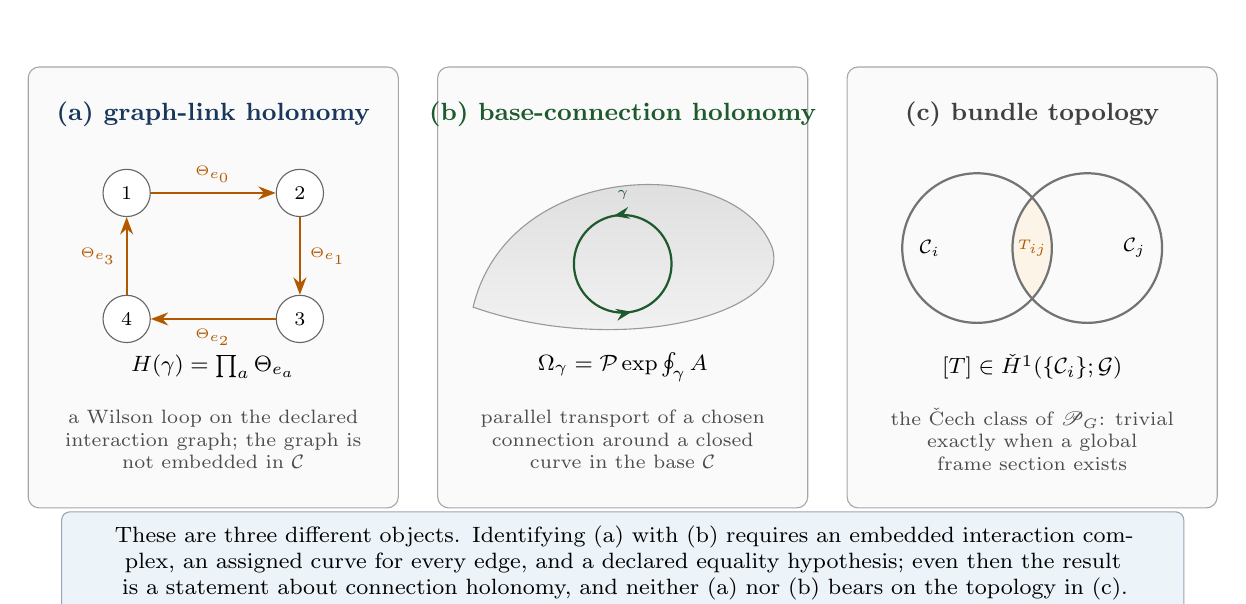
\begin{tikzpicture}[
  >={Stealth[length=2.2mm]},
  every node/.style={font=\small},
  panel/.style={draw=black!35, fill=black!2, rounded corners=4pt},
  nd/.style={draw=black!60, circle, fill=white, minimum size=6mm,
             inner sep=0pt, font=\scriptsize},
  ttl/.style={font=\small\bfseries, align=center},
  capt/.style={font=\scriptsize, align=center, text=black!70}
]
\node[panel, minimum width=4.7cm, minimum height=5.6cm] at (2.25,1.25) {};
\node[ttl, text=deepblue] at (2.25,3.45) {(a) graph-link holonomy};
\node[nd] (v1) at (1.15,2.45) {$1$};
\node[nd] (v2) at (3.35,2.45) {$2$};
\node[nd] (v3) at (3.35,0.85) {$3$};
\node[nd] (v4) at (1.15,0.85) {$4$};
\draw[->, thick, orange!70!black] (v1) -- node[above, font=\tiny]{$\Theta_{e_0}$} (v2);
\draw[->, thick, orange!70!black] (v2) -- node[right, font=\tiny]{$\Theta_{e_1}$} (v3);
\draw[->, thick, orange!70!black] (v3) -- node[below, font=\tiny]{$\Theta_{e_2}$} (v4);
\draw[->, thick, orange!70!black] (v4) -- node[left, font=\tiny]{$\Theta_{e_3}$} (v1);
\node[font=\footnotesize] at (2.25,0.24) {$H(\gamma)=\prod_a\Theta_{e_a}$};
\node[capt] at (2.25,-0.68)
  {a Wilson loop on the declared\\ interaction graph; the graph is\\
   not embedded in $\mathcal C$};
\node[panel, minimum width=4.7cm, minimum height=5.6cm] at (7.45,1.25) {};
\node[ttl, text=deepgreen] at (7.45,3.45) {(b) base-connection holonomy};
\shade[top color=black!14, bottom color=black!4, draw=black!40]
  (5.55,1.0) .. controls (6.0,2.9) and (8.9,2.95) .. (9.35,1.75)
  .. controls (9.6,0.9) and (7.4,0.35) .. (5.55,1.0) -- cycle;
\draw[thick, deepgreen, postaction={decorate, decoration={markings,
      mark=at position 0.28 with {\arrow{Stealth[length=2mm]}},
      mark=at position 0.78 with {\arrow{Stealth[length=2mm]}}}}]
  (7.45,1.55) circle (0.62);
\node[font=\tiny, text=deepgreen] at (7.45,2.42) {$\gamma$};
\node[font=\footnotesize] at (7.45,0.24) {$\Omega_\gamma=\mathcal P\exp\oint_\gamma A$};
\node[capt] at (7.45,-0.68)
  {parallel transport of a chosen\\ connection around a closed\\
   curve in the base $\mathcal C$};
\node[panel, minimum width=4.7cm, minimum height=5.6cm] at (12.65,1.25) {};
\node[ttl, text=black!75] at (12.65,3.45) {(c) bundle topology};
\begin{scope}
  \clip (11.95,1.75) circle (0.95);
  \fill[softorange] (13.35,1.75) circle (0.95);
\end{scope}
\draw[thick, black!55] (11.95,1.75) circle (0.95);
\draw[thick, black!55] (13.35,1.75) circle (0.95);
\node[font=\scriptsize] at (11.35,1.75) {$\mathcal C_i$};
\node[font=\scriptsize] at (13.95,1.75) {$\mathcal C_j$};
\node[font=\tiny, text=orange!70!black] at (12.65,1.75) {$T_{ij}$};
\node[font=\footnotesize] at (12.65,0.24) {$[T]\in\check H^1(\{\mathcal C_i\};\mathcal G)$};
\node[capt] at (12.65,-0.68)
  {the \v Cech class of $\mathscr P_G$: trivial\\ exactly when a global\\
   frame section exists};
\node[draw=deepblue!45, fill=softblue, rounded corners=3pt, align=center,
      font=\footnotesize, inner sep=5pt, text width=13.9cm] at (7.45,-2.25)
  {These are three different objects. Identifying (a) with (b) requires an embedded interaction
   complex, an assigned curve for every edge, and a declared equality hypothesis; even then the
   result is a statement about connection holonomy, and neither (a) nor (b) bears on the
   topology in (c).};
\end{tikzpicture}}
\caption{\textbf{Three holonomies.} The manuscript keeps graph-link holonomy, base-connection holonomy, and bundle topology strictly separate, and identifies them only under explicitly stated hypotheses. Almost every overreach the manuscript warns against consists of silently merging two of these panels.}
\label{fig:holonomy}
\end{figure}

The first is \emph{graph-link holonomy}. A finite interaction multigraph is declared independently of \(\mathcal C\), and to each oriented edge copy \(e:j\to i\) is attached a group element \(\Theta_e^x\) with \(\Theta_{\bar e}^x=(\Theta_e^x)^{-1}\). Under independent vertex reframings these transform as \(\Theta_e^{\prime}=(a_i)^{-1}\Theta_e a_j\), and the ordered product around a closed edge walk,
\begin{equation}
  H^x(\gamma)=\prod_{a=0}^{r-1}\Theta_{e_a}^x,
  \label{eq:graph-holonomy}
\end{equation}
has a gauge-invariant conjugacy class. This is exactly the lattice gauge theory situation: \(\Theta_e\) is a link variable, \(H(\gamma)\) is a Wilson loop, and the reframing law is the site-dependent gauge transformation. The manuscript's trivializing criterion is the lattice statement a physicist already knows: there exist vertex elements \(V_i\) with \(\Theta_e=V_iV_j^{-1}\) for every internal edge if and only if the ordered product around every closed internal walk is the identity. A link configuration is pure gauge precisely when all its Wilson loops are trivial.

The second is \emph{base-connection holonomy}. A chosen principal connection \(\omega_x\) has local potential \(A_i^x=(u_i^x)^*\omega_x\) obeying
\begin{equation}
  A_i^{\prime}=\Ad_{a_i^{-1}}A_i+a_i^{-1}da_i,
  \label{eq:gauge-potential}
\end{equation}
and its parallel transport around a closed curve \(\gamma\subset\mathcal C\) is the path-ordered exponential. This is the continuum Wilson loop.

The third is the \emph{topology of \(\mathscr P_G\)}, recorded by the \v Cech class of the transition cocycle \(T_{ij}\). The two frame atlases give cohomologous cocycles, so there is one class, and it is trivial exactly when a global frame section exists.

Nothing relates these three unless something is declared. The graph is not embedded in \(\mathcal C\), so \(\Theta_e\) is not a transport along any curve until an embedding, a curve assignment \(\gamma_e\), and the equalities \(\widehat\rho_b(\Theta_e^b)=\Omega_{\gamma_e}\) are hypothesized. Even under that hypothesis the conclusion concerns connection holonomy and says nothing about bundle topology. The manuscript's interpretation chapter makes the point sharply: the graph-link observable is not claimed to be evidence of base curvature or of bundle topology, and constructing a population observable sensitive to base holonomy is listed as an open problem with a precise specification of what would settle it.

\begin{translationbox}
On a lattice you have plaquette variables, in the continuum you have \(\mathcal P\exp\oint A\), and separately you have the instanton number of the bundle. A lattice gauge theorist knows these are three statements, that the second follows from the first only in a controlled classical continuum limit, and that neither determines the third. The manuscript enforces exactly that discipline, and most of its negative results are consequences of enforcing it.
\end{translationbox}

\section{The variational core}

\subsection{Evidence, the bound, and the gap}

On a finite design the theory declares one normalized generative joint over observations and latents, conditioned on structural data \(X\),
\begin{equation}
  \Prob_\theta:(X,\mathscr X)\longrightarrow\Law(\mathsf O_D\times\mathsf Y_D),
  \label{eq:generative-signature}
\end{equation}
built as an ordered composition of normalized Markov kernels along a topological order of the agent graph. Because each factor is separately normalized, the composition normalizes exactly and there is no partition function to compute. Separately it declares one correlated recognition law \(\Rec_X(dY\mid o)\), which is permitted to correlate agents with each other and the belief channel with the model channel; no factorization is imposed.

The exact identity is Equation~\eqref{eq:elbo-identity}. It says that the log evidence splits into a variational bound and a nonnegative gap, with equality exactly when the recognition law equals the posterior as a measure. Matching coordinate marginals is not enough.

For a physicist this is the Gibbs variational principle. Writing \(\log Z\) for the log evidence, \(\mathcal L\) for the bound, and the gap as a relative entropy of a trial state against the true conditional, Equation~\eqref{eq:elbo-identity} has the same content as
\begin{equation}
  -\beta F=\log Z\geq \log Z_0-\beta\langle H-H_0\rangle_0,
  \label{eq:gbf}
\end{equation}
with the difference between the two sides equal to \(\KL\) of the trial ensemble against the true one. Mean-field theory is the special case in which the trial state is taken to factorize; the manuscript's default is the opposite, since its recognition law is allowed to be fully correlated and the cost of factorizing is computed rather than ignored. That cost is a total correlation, and the manuscript records the exact chain identity relating the correlated and factorized bounds.

An energy presentation is available when the terms are separately finite,
\begin{equation}
  \mathcal F(\Rec)=\KL(\Rec\Vert P_0)+\Ex_{\Rec}H_o,
  \label{eq:energy-form}
\end{equation}
with \(H_o(y)=-\log L_o(y)\) the interaction energy of a configuration given the record. This is entropy against energy in the usual arrangement, and it is a derived representation rather than the definition, because at singular trial laws the two terms can be separately infinite while their difference is not.

\subsection{Why the model may not read the belief}

A restriction that looks pedantic on first encounter turns out to be load bearing, and it has a clean physical reading. The arguments of every generative factor are the parameters \(\theta\) and the structural data \(X\), and nothing else. No factor of the generative law may take as an argument the recognition law, one of its marginals or parameters, or a posterior.

The reason is that the variational principle certifies an improvement in a \emph{fixed} quantity. If a generative factor is indexed by a nonconstant family of recognition laws, then the joint moves whenever the inference moves, and the family selects no joint as the model, so there is no fixed evidence to bound. The manuscript proves this rather than asserting it, and supplies a finite binary witness showing that the naive intuitions about how such a scheme would fail are themselves wrong: the failure is not a monotonicity failure but the absence of a fixed target.

\begin{physicalreading}
You may not let the Hamiltonian depend on your trial density matrix and still call the result a variational bound. The bound would be on a moving target, and no sequence of improvements would certify anything about a fixed free energy. Everything downstream in the manuscript, including the renormalization statements, depends on the generative law being frozen before recognition is chosen.
\end{physicalreading}

Two constructions that superficially resemble a violation are explicitly cleared. A posterior that flows with an information-theoretic scale, as in Bayesian renormalization, is the output of a declared Bayesian model, and allowing it to flow does not make a generative kernel read its own posterior. What is not permitted is to take a posterior from one scale and insert it as the generative top factor at another without declaring either a new model at each scale or an explicit transition rule, since the evidence and bound at different scales would then refer to different joints. Similarly, a loop in an inference algorithm is not a cycle in the factorization of the model, a distinction that becomes the substance of the no-go result in Section~\ref{sec:nogo}.

\subsection{Infinite penalties are real penalties}

Relative entropy here is defined on the extended reals: it is the integral of the log density ratio when the numerator is absolutely continuous with respect to the denominator, and \(+\infty\) otherwise. The manuscript proves a consequence that matters in practice. If the posterior is dominated by Lebesgue measure on \(\mathbb R^d\) while the recognition law is supported on a proper affine subspace, then that subspace carries posterior mass zero and recognition mass one, so the divergence is infinite outright. The relevant sentence in the manuscript is that the cost is not a large finite number to be traded against something else but an infinite one.

This is the exact mechanism that forbids degenerate recognition families, for example any family that ties several latents to one shared value. A physicist should read it as the statement that a trial ensemble supported on a measure-zero set of configurations has no finite free energy relative to a nondegenerate reference, and that no amount of energetic gain compensates.

\section{Many agents}

\subsection{One collective free energy, and local descent on it}

For a finite agent hypergraph with normalized interaction-record kernels, the complete record density factorizes over records,
\begin{equation}
  \ell(o\mid y)=\prod_{a\in\mathcal A}\ell_a(o_a\mid y_{\partial a}),
  \qquad
  H_o(y)=\sum_{a\in\mathcal A}-\log\ell_a(o_a\mid y_{\partial a}),
  \label{eq:record-factorization}
\end{equation}
where \(\partial a\) is the scope of record \(a\). There is one term per actual record, so an undirected record shared by two agents occurs once; writing both \(E_{ij}\) and \(E_{ji}\) asserts two directed records rather than two descriptions of one.

For every trial law \(Q\) the collective free energy is
\begin{equation}
  \mathcal F_o(Q)=-\log Z(o)+\KL(Q\Vert\Pi_o),
  \label{eq:collective-vfe}
\end{equation}
and for a nonempty block \(B\), conditioning on the outside state \(b=y_{B^c}\) gives a block free energy \(\mathcal F_{B,o}(r_B;b)\) of exactly the same form, built from the records incident to \(B\). The singleton \(B=\{i\}\) is one agent and a larger \(B\) is a meta-agent; the construction does not change.

The result that organizes the multi-agent theory is an exact potential identity. If two trial laws share the same outside marginal and both have finite divergence against the posterior, then
\begin{equation}
  \mathcal F_o(Q')-\mathcal F_o(Q)
  =\Ex_{Q_{B^c}}\left[\mathcal F_{B,o}(r'_B;Y_{B^c})-\mathcal F_{B,o}(r_B;Y_{B^c})\right].
  \label{eq:local-global}
\end{equation}
Every exact local conditional update is therefore a coordinate update of the one collective free energy. The proof is a relative-entropy chain rule; the outside terms agree and cancel, and so does the local log normalizer.

Two consequences deserve emphasis. The identity licenses sequential exact coordinate minimization, damped updates accepted by the collective objective, and continuous block-gradient dynamics. It does \emph{not} license replacing all correlated full conditionals in parallel, because independently replacing them need not define any joint recognition law at all. Separately, the local objectives do not sum to the collective one, because a record whose scope meets several blocks appears in every incident local objective; additive accounting across agents is a different construction with a total-correlation correction.

\begin{physicalreading}
This is the cavity or block mean-field arrangement made exact. There is one Landau-type functional on the joint trial law, each block's local free energy is the conditional free energy of that block in the field of the rest, and block-coordinate descent is exact descent on the global functional. The failure of parallel updates is the familiar failure of simultaneously replacing every spin by its cavity field.
\end{physicalreading}

\subsection{Attention as a Boltzmann weight over sources}

The theory accommodates attention without violating the typing prohibition, by putting a latent source label inside the fixed joint. For each receiving agent \(i\), a categorical latent \(J_i\) with prior \(\pi_i\) augments the baseline, and the record likelihood is declared to carry a source-dependent energy,
\begin{equation}
  \ell_i(o_i\mid y,J_i=j)=c_i(o_i,y)\exp\bigl[-D_{ij}(y)/\tau_i\bigr],
  \label{eq:attention-likelihood}
\end{equation}
where \(D_{ij}\) is a fixed gauge-invariant function of latent states and declared transports and contains no live recognition distribution. Bayes' rule then gives the generative posterior row
\begin{equation}
  \beta^P_{ij}(y)=\frac{\pi_{ij}\exp[-D_{ij}(y)/\tau_i]}{\sum_k\pi_{ik}\exp[-D_{ik}(y)/\tau_i]},
  \label{eq:attention-posterior}
\end{equation}
and, after restricting the recognition law so that each row is independent of the latent state, the exact dimensionless row contribution to the collective free energy is
\begin{equation}
  \mathcal F_i^{\mathrm{att}}(\beta_i)=\KL(\beta_i\Vert\pi_i)
  +\frac{1}{\tau_i}\sum_j\beta_{ij}\Ex_{Q_Y}D_{ij},
  \label{eq:attention-vfe}
\end{equation}
where \(\overline D_{ij}:=\Ex_{Q_Y}D_{ij}\). In the same energy units as \(D_{ij}\), the physically transparent row free energy is
\begin{equation}
  \boxed{\mathcal F_i^{\mathrm{row}}(\beta_i)
  :=\tau_i\mathcal F_i^{\mathrm{att}}(\beta_i)
  =\sum_j\beta_{ij}\overline D_{ij}
  +\tau_i\KL(\beta_i\Vert\pi_i).}
  \label{eq:attention-row-free-energy}
\end{equation}
The relative-entropy term contains both the source entropy and the reference weight,
\begin{equation}
  \tau_i\KL(\beta_i\Vert\pi_i)
  =-\tau_i S(\beta_i)-\tau_i\sum_j\beta_{ij}\log\pi_{ij}.
  \label{eq:row-helmholtz-split}
\end{equation}
For a uniform prior the final term is constant, leaving the literal canonical form \(U_i-\tau_iS_i\). For a nonuniform prior, \(\pi_i\) acts as a reference degeneracy or prior field.

The unique interior minimizer is
\begin{equation}
  \beta_{ij}^{\star}
  =\frac{\pi_{ij}\exp(-\overline D_{ij}/\tau_i)}{Z_i},
  \qquad
  Z_i=\sum_k\pi_{ik}\exp(-\overline D_{ik}/\tau_i),
  \label{eq:attention-row-optimum}
\end{equation}
and the reduced values are
\begin{equation}
  \mathcal F_{i,\mathrm{red}}^{\mathrm{row}}=-\tau_i\log Z_i,
  \qquad
  \mathcal F_{i,\mathrm{red}}^{\mathrm{att}}=-\log Z_i.
  \label{eq:attention-row-reduced}
\end{equation}
Thus softmax is the equilibrium distribution of a canonical ensemble over sources, not merely an architectural choice. The two functionals have the same minimizer, but the distinction matters globally: multiplying one row sector by \(\tau_i\) does not produce another standard ELBO unless the whole objective is rescaled or a generalized free energy is separately declared.

The dynamics is equally recognizable. Holding the latent recognition law fixed, the Fisher natural gradient of \eqref{eq:attention-vfe} on the open simplex is the replicator equation
\begin{equation}
  \dot\beta_{ij}=-\gamma_i\beta_{ij}\Bigl(c_{ij}-\sum_k\beta_{ik}c_{ik}\Bigr),
  \qquad
  c_{ij}=\log\frac{\beta_{ij}}{\pi_{ij}}+\frac{\Ex_{Q_Y}D_{ij}}{\tau_i},
  \label{eq:replicator}
\end{equation}
with partial dimensionless rate \(-\gamma_i\operatorname{Var}_{\beta_i}(c_{ij})\leq0\). In row-energy units, and with \(\tau_i\) and \(\pi_i\) fixed, the beta-only and full rates are
\begin{align}
  \left.\frac{d\mathcal F_i^{\mathrm{row}}}{dt}\right|_{\beta_i}
  &=-\gamma_i\tau_i\operatorname{Var}_{\beta_i}(c_{ij}),
  \nonumber\\
  \frac{d\mathcal F_i^{\mathrm{row}}}{dt}
  &=-\gamma_i\tau_i\operatorname{Var}_{\beta_i}(c_{ij})
  +\sum_j\beta_{ij}\frac{d\overline D_{ij}}{dt}.
  \label{eq:attention-row-total-rate}
\end{align}
The second term is the missing piece when beliefs, transports, or both evolve. Coevolving \(\beta_{ij}\) and \(D_{ij}\) is therefore an annealed network, but row descent alone does not prove descent of the coupled system. Every evolving variable must follow the derivative of one common scalar. If the row is kept at its instantaneous optimum, the envelope theorem gives
\begin{equation}
  \frac{d\mathcal F_{i,\mathrm{red}}^{\mathrm{row}}}{dt}
  =\sum_j\beta_{ij}^{\star}\frac{d\overline D_{ij}}{dt}.
  \label{eq:attention-row-envelope}
\end{equation}
The variance dissipation has the same mathematical shape as Fisher's fundamental theorem; it is not a theorem about biological fitness.

\begin{boundarybox}
The clean softmax requires two declared hypotheses, and the manuscript states both. The augmented likelihood must factor so that no other record reads a source label, and the recognition law must factor over rows with each row independent of the latent state. Without the first, an extra label-dependent factor enters Bayes' rule and changes the answer. Without the second, a correlated conditional law retains a nonnegative conditional total-correlation term, and a row softmax is not asserted. The two softmax rows also answer different questions: the recognition optimum is generally not the recognition average of the pointwise posterior row, and the two agree only when the energy differences are almost surely constant.
\end{boundarybox}

\section{Thermodynamic hierarchy: adaptive bonds, grand occupation, and parent formation}
\label{sec:thermodynamic-hierarchy}

\subsection{Why variational free energy has the Helmholtz form}

The word ``free energy'' is not merely metaphorical, but its exact content is information theoretic before it is physical. For a fixed normalized joint \(p_\theta(o,y\mid X)\), define the dimensionless configuration energy \(E_o(y):=-\log p_\theta(o,y\mid X)\). Then the variational free energy is
\begin{equation}
  \mathcal F[Q]
  =\Ex_Q E_o(Y)-S[Q]
  =\KL(Q\Vert\Post_{o,X})-\log p_\theta(o\mid X),
  \label{eq:vfe-helmholtz}
\end{equation}
where \(S[Q]=-\Ex_Q\log q(Y)\) when a common density representation is available. Equation~\eqref{eq:vfe-helmholtz} is the Gibbs variational functional with Helmholtz form \(U-TS\) in units with \(k_B T=1\). Introducing an explicit information-temperature scale gives \(\mathcal F_T=U-TS\), and minimizing over \(Q\) gives the negative log-partition value. This is the structural reason for Friston's terminology, and it is the same maximum-entropy calculus used by Jaynes \cite{Friston2010,Jaynes1957}.

The correspondence does not by itself identify \(-\log p\) with a physical Hamiltonian, \(S[Q]\) with thermodynamic entropy in joules per kelvin, or the descent parameter with time. Those identifications require a physical energy scale, a reservoir or environment, and an accounting of heat, work, and entropy production. The main manuscript proves the normalized probabilistic identity and uses the thermodynamic dictionary as an interpretation; it does not derive physical thermodynamics from probability theory.

\begin{physicalreading}
The exact statement is that VFE is a Gibbs variational functional with Helmholtz form over trial probability laws. The additional statement that this functional is the thermodynamic free energy of a physical system is a model-dependent hypothesis. Information temperature, physical temperature, inference time, and laboratory time must not be identified without an operational map.
\end{physicalreading}

\subsection{The fine-agent network before any meta-agent exists}

Before coarse graining, the population contains only fine agents and their possible communication channels. A useful reduced presentation of the belief sector is
\begin{align}
  \mathcal F_{\mathrm{net}}
  &=\sum_i\left[
    \alpha_i\KL(q_i\Vert p_i)
    -\Ex_{q_i}\log p(o_i\mid c_i)
  \right]
  \nonumber\\
  &\quad+\sum_i\left[
    \sum_j\beta_{ij}D_{ij}
    +\tau_i\KL(\beta_i\Vert\pi_i)
  \right],
  \qquad
  D_{ij}=\KL\bigl(q_i\Vert(\Omega_{ij})_{\#}q_j\bigr).
  \label{eq:reduced-network-free-energy}
\end{align}
Here \(\alpha_i\) weights the self-prior sector, while \(\beta_{ij}\) is a normalized source row; it is unrelated to the thermodynamic convention in which a bare \(\beta\) denotes inverse temperature. The detailed manuscript obtains the attention term from a fixed normalized joint by adjoining a latent source label. Equation~\eqref{eq:reduced-network-free-energy} should therefore be read as a reduced network sector whose exact fixed-joint status depends on the hypotheses already stated above, not as a license to let a generative kernel read a live peer belief.

When \(q_i\), \(\Omega_{ij}\), and \(\beta_{ij}\) all evolve, the network is annealed: both the configurations and the effective bonds respond. Low transported mismatch can attract attention, and increased attention can strengthen the forces reducing mismatch. This feedback may form a coherent subgraph. It has not yet created a parent latent, a parent generative law, or a parent posterior, so coherence alone is not meta-agent construction.

\subsection{Why the attention--mismatch product is not yet a chemical-potential law}

The tempting algebra is real. At one instant, setting \(N_{ij}:=D_{ij}\) and \(\mu_{ij}:=-\beta_{ij}\) gives
\begin{equation}
  \beta_{ij}D_{ij}=-\mu_{ij}N_{ij},
  \qquad
  d(\beta_{ij}D_{ij})
  =-N_{ij}d\mu_{ij}-\mu_{ij}dN_{ij}.
  \label{eq:formal-chemical-potential-map}
\end{equation}
The equality remains algebraically true when both factors change. Its thermodynamic interpretation does not follow. The row weight \(\beta_{ij}\) is constrained by \(\sum_j\beta_{ij}=1\), is learned from the state, and is not an externally imposed intensive field. The divergence \(D_{ij}\) is generally neither an extensive count nor a conserved quantity exchanged with a reservoir. The full row objective also contains the entropy term, whose derivative is omitted by the bare product. Equation~\eqref{eq:formal-chemical-potential-map} is therefore a Legendre-shaped relabeling, not yet the grand potential of the agent network.

This distinction answers what changes when both \(\beta_{ij}\) and \(D_{ij}\) descend. Their product has two chain-rule terms, but the canonical row has the additional entropy derivative shown in Equation~\eqref{eq:attention-row-total-rate}. If all variables follow the full derivative of one time-independent scalar, that scalar is Lyapunov. If each sector follows a separately truncated force, or if the external controls change, monotone descent is no longer implied.

\subsection{A genuine grand-canonical topology}

\begin{proposalbox}
A true grand-canonical extension introduces a binary edge occupation \(a_{ij}\in\{0,1\}\), its mean \(\rho_{ij}=\Ex[a_{ij}]\), and a chemical potential \(\mu_{ij}\) conjugate to the edge count. This extension is developed in \path{Theory/grand_canonical_meta_agent_formation.tex}; it is not part of the established target of \path{Theory/main.tex}.
\end{proposalbox}

Let \(\pi_{ij}^{E}\in(0,1)\) be a reference edge occupation and let \(\epsilon_{ij}\) contain gauge-invariant belief mismatch, model mismatch, boundary cost, and any declared retention gain. The independent-edge grand functional is
\begin{align}
  \mathcal G[q,\rho]
  &=\mathcal F_{\mathrm{agents}}[q]
  +\sum_{ij}\rho_{ij}\epsilon_{ij}[q]
  -\sum_{ij}\mu_{ij}\rho_{ij}
  \nonumber\\
  &\quad+\tau_E\sum_{ij}
  \KL\bigl(\mathrm{Bern}(\rho_{ij})\Vert
            \mathrm{Bern}(\pi_{ij}^{E})\bigr).
  \label{eq:grand-edge-functional}
\end{align}
Write \(\Phi_E\) for the edge-sector functional after minimization over \(\rho\), with all other variables fixed. Its unique occupation is
\begin{equation}
  \rho_{ij}^{\star}
  =\left[
    1+\frac{1-\pi_{ij}^{E}}{\pi_{ij}^{E}}
    \exp\left(\frac{\epsilon_{ij}-\mu_{ij}}{\tau_E}\right)
  \right]^{-1},
  \qquad
  -\frac{\partial\Phi_E}{\partial\mu_{ij}}=\rho_{ij}^{\star}.
  \label{eq:grand-edge-occupation}
\end{equation}
This is a literal lattice-gas or Fermi occupation law on a network \cite{ParkNewman2004}. The variable \(\rho_{ij}\) answers whether an edge exists; \(\beta_{ij}\) answers which admitted source is selected conditional on a receiver event. Their roles coincide only after an additional normalization convention, and even then the count-bearing quantity is the unnormalized expected degree, not the row itself.

Under fixed chemical potentials, temperatures, records, and boundary data, a joint natural-gradient flow of beliefs, frames, and Bernoulli occupations descends \(\mathcal G\) when every sector uses the full derivative of this same scalar. Driven reservoirs add work terms such as \(-\sum_{ij}\rho_{ij}\dot\mu_{ij}\). Sustained nonequilibrium then requires an open flux, explicit time-dependent drive, stochastic forcing, delay, nonreciprocity, or an antisymmetric kinetic sector. Adaptive coevolution alone can yield metastability and long transients, but fixed-control gradient flow still relaxes \cite{GrossBlasius2008}.

\subsection{From a coherent cluster to a pointwise parent}

The established meta-agent result begins after a nonempty child block \(I\), a parent label \(A\), and one normalized recognition-independent coarse channel \(C_A:\mathsf Y_I\rightsquigarrow\mathsf Z_A\) have been declared. The observation and structural input remain outside the random channel. The full pointwise parent datum is
\begin{equation}
  \Prob_A=(\id_{\mathsf O}\times C_A)_{\#}\Prob_I,
  \qquad
  \Rec_A=(C_A)_{\#}\Rec_I,
  \qquad
  \Post_{A,o,X}=(C_A)_{\#}\Post_{I,o,X}.
  \label{eq:parent-full-triple}
\end{equation}
The parent belief and model laws are projections or disintegrations of these full laws. Constructing two consensus marginals does not reconstruct the parent joint, its posterior, or its VFE.

The exact information accounting is
\begin{equation}
  \KL(\Rec_I\Vert\Post_I)
  =\KL(\Rec_A\Vert\Post_A)+\Delta_A,
  \qquad
  \Delta_A=\int\KL(\widehat\Rec_I(\cdot\mid z)
  \Vert\widehat\Post_I(\cdot\mid z))\Rec_A(dz),
  \label{eq:parent-kl-defect}
\end{equation}
as an additive identity in \([0,+\infty]\). Adding the same finite evidence term gives the extended-real VFE identity. Ordinary subtraction and the two-way recovery criterion require finite fine KL. A parent may therefore discard most microscopic information, as a university ignores most detailed states of its members, while retaining a declared interface; \(\Delta_A\) measures the recognition-relevant information lost by that declaration.

\begin{figure}[ht]
\centering
\resizebox{\textwidth}{!}{%
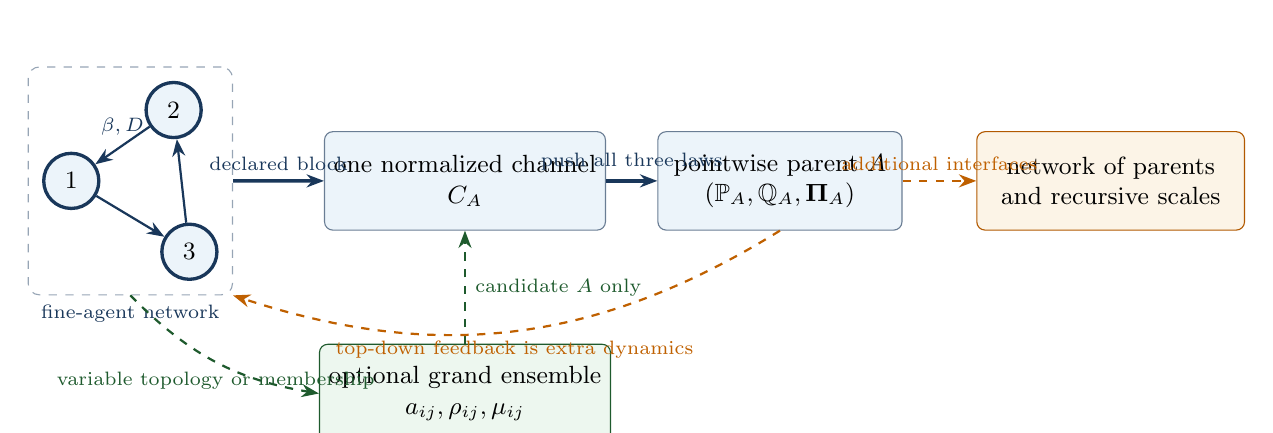
\begin{tikzpicture}[
  >={Stealth[length=2.2mm]},
  every node/.style={font=\small},
  ag/.style={circle, draw=deepblue, very thick, fill=softblue, minimum size=7mm},
  box/.style={draw=deepblue!65, fill=softblue, rounded corners=3pt, align=center, minimum width=3.1cm, minimum height=1.25cm},
  prop/.style={draw=deepgreen, fill=softgreen, rounded corners=3pt, align=center, minimum width=3.3cm, minimum height=1.25cm},
  open/.style={draw=orange!70!black, fill=softorange, rounded corners=3pt, align=center, minimum width=3.4cm, minimum height=1.25cm}
]
\node[ag] (a1) at (0,1.1) {$1$};
\node[ag] (a2) at (1.3,2.0) {$2$};
\node[ag] (a3) at (1.5,0.2) {$3$};
\draw[->, thick, deepblue] (a2) -- node[above, font=\scriptsize] {$\beta,D$} (a1);
\draw[->, thick, deepblue] (a3) -- (a2);
\draw[->, thick, deepblue] (a1) -- (a3);
\node[draw=deepblue!45, dashed, rounded corners, fit=(a1)(a2)(a3), inner sep=5pt,
      label={[font=\scriptsize, text=deepblue]below:fine-agent network}] (fine) {};
\node[box] (channel) at (5.0,1.1) {one normalized channel\\$C_A$};
\node[box] (parent) at (9.0,1.1) {pointwise parent $A$\\$(\Prob_A,\Rec_A,\Post_A)$};
\node[open] (tower) at (13.2,1.1) {network of parents\\and recursive scales};
\node[prop] (grand) at (5.0,-1.6) {optional grand ensemble\\$a_{ij},\rho_{ij},\mu_{ij}$};
\draw[->, very thick, deepblue] (fine.east) -- node[above, font=\scriptsize] {declared block} (channel.west);
\draw[->, very thick, deepblue] (channel) -- node[above, font=\scriptsize] {push all three laws} (parent);
\draw[->, thick, dashed, orange!75!black] (parent) -- node[above, font=\scriptsize] {additional interfaces} (tower);
\draw[->, thick, dashed, deepgreen] (fine.south) to[bend right=18]
  node[below, font=\scriptsize] {variable topology or membership} (grand.west);
\draw[->, thick, dashed, deepgreen] (grand) -- node[right, font=\scriptsize] {candidate $A$ only} (channel.south);
\draw[->, thick, dashed, orange!75!black] (parent.south) to[bend left=25]
  node[below, font=\scriptsize] {top-down feedback is extra dynamics} (fine.south east);
\end{tikzpicture}}
\caption{\textbf{Four logically separate stages.} Canonical attention can reorganize a fine-agent network without changing edge number. A proposed grand ensemble can select variable edges or candidate memberships, but it does not itself construct a parent. The established pointwise theorem begins with one declared channel and pushes the complete law triple. Networks of parents, cross-scale feedback, and recursive dynamics require additional interfaces and dynamical hypotheses.}
\label{fig:thermodynamic-hierarchy}
\end{figure}

\subsection{Trees pool, loops obstruct: how a parent is actually assembled}
\label{sec:trees-loops}

Readers meeting the parent construction often ask why it runs on a spanning tree when the
interesting geometry lives on the loops. The two are not competing mechanisms; they are the
constructive half and the obstruction half of one operation, and keeping their roles separate is
what the stabilizer condition is for. Figure~\ref{fig:trees-loops} draws the division of labor.

Start with the comparison problem. Each member $i$ of a block $I$ holds its belief $q_i$ in its
own frame, and pooling requires expressing every member in one frame. An edge $(i\!\leftarrow\!j)$
carries the declared transport $\Omega_{ij}$, so any path $P$ from $i$ to a chosen root $r$
defines a composite transport, the ordered product along the path,
\begin{equation}
  \Omega_{r\leftarrow i}[P]=\prod_{e\in P}\Omega_e^{\pm 1},
  \label{eq:tree-transport}
\end{equation}
and the pooled parent presentation is built from the transported beliefs
$\Omega_{r\leftarrow i}\,q_i$. The problem is that different paths need not agree. Choosing a
spanning tree $T$ selects one path per member and makes \eqref{eq:tree-transport} well defined;
this is not an approximation but a \emph{gauge choice}, the maximal-tree gauge fixing standard in
lattice gauge theory since Wilson~\cite{Wilson1974}: along tree edges the transports can be
absorbed into frame redefinitions, and every physical degree of freedom that remains lives on the
edges the tree omits~\cite{Kogut1979}.

Those omitted edges are exactly where the loops enter. Each non-tree edge $e$ closes one
fundamental loop $\ell_e$ against the tree, with holonomy
\begin{equation}
  H_{\ell_e}=\Omega_{r\leftarrow j}\,\Omega_e\,\Omega_{r\leftarrow i}^{-1},
  \qquad e=(i\!\leftarrow\!j),
  \label{eq:loop-holonomy}
\end{equation}
the loop transport expressed at the root, and the group generated by these elements is the
block's based holonomy group $\mathrm{Hol}_r(I)$. Plaquette curvature is the same content
localized on faces. The tree cannot flatten any of this; what it can do is make the question
precise. The pooled parent is path independent, so that the tree's arbitrariness was harmless,
exactly when the pooled presentation is fixed by every loop transport,
\begin{equation}
  H\,\#\,\bar q_I=\bar q_I
  \qquad\text{for every } H\in\mathrm{Hol}_r(I),
  \label{eq:stabilizer-condition}
\end{equation}
which is the stabilizer condition. When \eqref{eq:stabilizer-condition} holds, a holonomy-blind
parent is legitimate: any path would have produced the same pooled target. When it fails, the
theory offers a disjunction rather than a prohibition. The stabilized route refuses the parent.
The retention route forms it anyway and makes it carry the obstruction as internal data, the
\emph{marks}: the root presentation, the holonomy generators, and the dressed boundary
generators
\begin{equation}
  V_e=\Omega_{r\leftarrow i}\,\Theta_e\,\Omega_{r'\leftarrow j}^{-1}
  \label{eq:dressed-boundary}
\end{equation}
for edges leaving the block, all kept as one root-gauge orbit and priced by a declared capacity
charge. Loops therefore act three times, never as the pooling mechanism: as the obstruction test
\eqref{eq:stabilizer-condition}, as an energy price through the plaquette term, and as the
retained record that the 2026-08-17 measurements showed is load-bearing, since the coarse links
between parents are composed from the boundary marks and the Wilson charge is conserved only
because the interior generators ride along.

\begin{figure}[ht]
\centering
\resizebox{0.98\textwidth}{!}{%
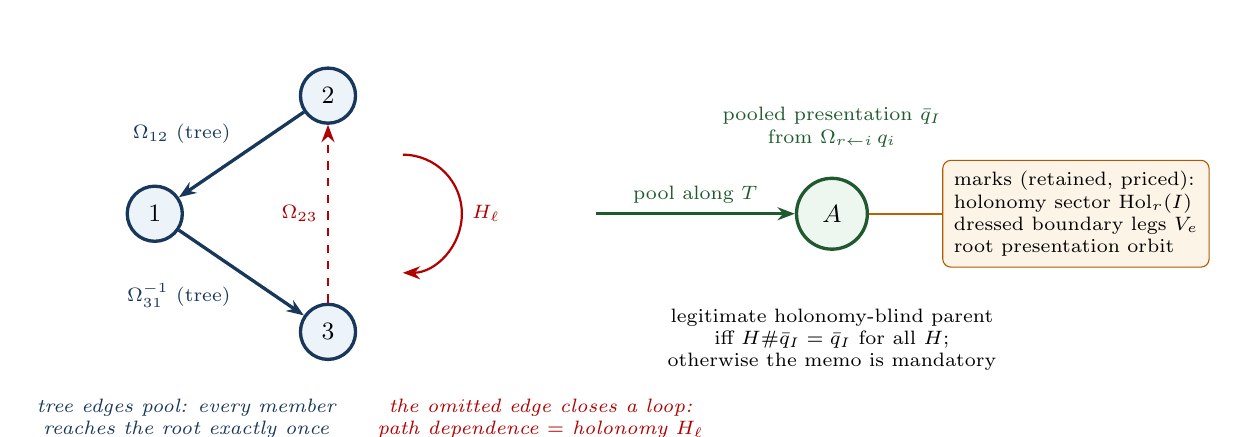
\begin{tikzpicture}[
  >={Stealth[length=2.2mm]},
  every node/.style={font=\small},
  ag/.style={circle, draw=deepblue, very thick, fill=softblue, minimum size=7mm},
  memo/.style={draw=orange!70!black, fill=softorange, rounded corners=3pt, align=left, font=\scriptsize, inner sep=4pt}
]
\node[ag] (b1) at (0,0) {$1$};
\node[ag] (b2) at (2.2,1.5) {$2$};
\node[ag] (b3) at (2.2,-1.5) {$3$};
\draw[->, very thick, deepblue] (b2) -- node[above left, font=\scriptsize] {$\Omega_{12}$ (tree)} (b1);
\draw[->, very thick, deepblue] (b1) -- node[below left, font=\scriptsize] {$\Omega_{31}^{-1}$ (tree)} (b3);
\draw[->, thick, dashed, red!70!black] (b3) -- node[left, font=\scriptsize] {$\Omega_{23}$} (b2);
\draw[->, thick, red!70!black] (3.15,0.75) arc[start angle=90, end angle=-90, radius=0.75]
  node[midway, right, font=\scriptsize] {$H_{\ell}$};
\node[font=\scriptsize\itshape, text=deepblue, align=center] at (0.4,-2.6)
  {tree edges pool: every member\\reaches the root exactly once};
\node[font=\scriptsize\itshape, text=red!70!black, align=center] at (4.9,-2.6)
  {the omitted edge closes a loop:\\path dependence $=$ holonomy $H_\ell$};
\node[ag, minimum size=9mm, fill=softgreen, draw=deepgreen] (parent) at (8.6,0) {$A$};
\node[font=\scriptsize, align=center, text=deepgreen] at (8.6,1.1)
  {pooled presentation $\bar q_I$\\from $\Omega_{r\leftarrow i}\,q_i$};
\node[memo, anchor=west] (marks) at (10.0,0)
  {marks (retained, priced):\\
   holonomy sector $\mathrm{Hol}_r(I)$\\
   dressed boundary legs $V_e$\\
   root presentation orbit};
\draw[->, very thick, deepgreen] (5.6,0) -- node[above, font=\scriptsize] {pool along $T$} (parent);
\draw[thick, orange!75!black] (parent) -- (marks);
\node[font=\scriptsize, align=center] at (8.6,-1.6)
  {legitimate holonomy-blind parent\\ iff $H\#\bar q_I=\bar q_I$ for all $H$;\\
   otherwise the memo is mandatory};
\end{tikzpicture}}
\caption{\textbf{Trees pool, loops obstruct.} A spanning tree (solid) gives each member exactly
one transport to the root, which is what makes pooling well defined; it is a gauge choice, not an
approximation. Each omitted edge (dashed) closes a loop whose root-framed transport
$H_\ell$ measures the path dependence the tree hid. The parent is the pooled presentation
together with, whenever the stabilizer condition \eqref{eq:stabilizer-condition} fails, the
retained marks: the holonomy sector and the dressed boundary generators.}
\label{fig:trees-loops}
\end{figure}

\begin{physicalreading}
The Cooper pair is the exact physical picture of a mark-carrying parent. Two spin-$\tfrac12$
electrons have a four-dimensional joint fiber, but the physically meaningful parent label is not
a point in that product: it is the decomposition into irreducible sectors of the symmetry acting
on the pair, singlet plus triplet, $\mathbf 2\otimes\mathbf 2=\mathbf 1\oplus\mathbf 3$. The
sector label is precisely what no transport can change, and the state within a sector is the
parent's internal presentation. In this theory's language: marks are the sector label, the
pooled presentation is the within-sector state, and the retention price is the capacity spent
carrying the label. The general pattern for fiber growth follows: a block's joint fiber grows
exponentially with block size, the way $N$ spins give $2^N$ states, while a legitimate parent
fiber is the sector decomposition, larger than one child's fiber but far smaller than the
joint. The finite laboratory currently pins the parent fiber to the child's, the block-spin
convention in which an Ising block spin is still $\pm1$, and the measured saturation of pair
retention at thickened boundaries is plausibly the cost of that pin; the declared capacity
experiment, enlarging the parent to presentation-times-sector, is the singlet/triplet idea run
as a measurement.
\end{physicalreading}

Two references cover the tree-versus-loop division in its original habitat: Wilson's
confinement paper introduces the link variables and loop observables themselves~\cite{Wilson1974},
and Kogut's review develops maximal-tree gauge fixing and the counting of physical degrees of
freedom on the omitted edges~\cite{Kogut1979}.

\subsection{Networks of meta-agents and participatory nonequilibrium}

Once several parents carry full probabilistic data and retained boundary interfaces, they may be treated as nodes of another declared network. That move does not follow merely by averaging the fine beliefs. Each scale needs its own normalized generative law, recognition law, posterior version, attention or edge variables, and comparison map to neighboring scales. Iteration produces a scale diagram; an RG flow additionally needs the rescalings and fixed reference object described later in this companion.

A grand-canonical membership sector can make expected parent size fluctuate under a membership chemical potential, and the construction can be repeated at higher levels. This is a proposed organization principle rather than a theorem selecting one hierarchy. The current main manuscript leaves canonical channel selection, partition selection, local-section gluing, overlapping memberships, and the construction of a geometric meta-agent open.

The Wheelerian possibility enters only when the parent changes the fine dynamics that sustain it. For a deterministic fine vector field \(V_t\), moving coarse map \(c_t\), and candidate parent field \(\overline V_t\), the semiconjugacy defect is
\begin{equation}
  \delta_t=\partial_t c_t+Dc_t V_t-\overline V_t\circ c_t.
  \label{eq:participatory-semiconjugacy-defect}
\end{equation}
Vanishing \(\delta_t\) gives trajectory semiconjugacy under the required regularity hypotheses; it does not by itself give autonomy. A participatory nonequilibrium model must also identify the reciprocal operators, account for work and flux without double counting, and supply an observable distinguishing its feedback from an ordinary hierarchical latent-variable model.

\begin{boundarybox}
The static pointwise parent theorem is established. Grand-canonical edge or membership occupation, a recursive network of probabilistic parents, cross-scale feedback, sustained nonequilibrium, and emergent agency are proposed or open. None follows from the notation \(U-TS-\mu N\) alone.
\end{boundarybox}

\section{Information geometry on the base}

The Fisher metric enters as the Hessian of an exponential-family log partition function, which is to say as a susceptibility: the second derivative of a free energy with respect to natural parameters, equal to the covariance of the sufficient statistics. That is the fluctuation-response relation, and it is the reason the metric is available at all.

The construction that makes this geometric is a pullback. A chosen connection splits the tangent space of an associated bundle into horizontal and vertical parts, so a smooth section \(s\) over an open subset of the base has a vertical first jet
\begin{equation}
  D^\omega s=\operatorname{ver}^\omega\circ Ts,
  \label{eq:covariant-jet}
\end{equation}
a vertical-valued one-form along \(s\). Feeding it into the fiberwise Fisher and Amari tensors gives symmetric tensors on the base itself,
\begin{equation}
  h_s^\omega(X,Y)=g^F_{s(c)}\bigl(D^\omega s(X),D^\omega s(Y)\bigr),
  \qquad
  c_s^\omega(X,Y,Z)=\mathcal T_{s(c)}\bigl(D^\omega s(X),D^\omega s(Y),D^\omega s(Z)\bigr).
  \label{eq:pullbacks}
\end{equation}
These are gauge covariant: two coordinate descriptions of the same connection-section pair give the same tensor.

Three qualifications travel with this result and the manuscript repeats them whenever the tensors are used. Passive covariance is not connection independence, and two different connections generally give different pullbacks, with an exact change formula recorded. Passive covariance is also not invariance under the active gauge group at fixed connection, and an explicit counterexample is given in which a bundle automorphism carries a section with vanishing pullback to one whose pullback is \(dx^2\). Finally, the Fisher pullback can be degenerate, so contextual directions can be left unmeasured, and the object is a semimetric until nondegeneracy is proved in a specific case.

\begin{translationbox}
This is an induced metric, in the sense in which a field configuration induces a metric on a worldvolume, rather than an intrinsic geometry of the base. It depends on the section, on the connection, and on the choice of Fisher metric in the fiber. No canonical connection is derived anywhere in the manuscript, so every statement about base geometry is relative to declared data.
\end{translationbox}

A related discipline governs what counts as an invariant. In the Gaussian realization the assembled precision splits as \(\Lambda=L+A\) into an interaction part and self terms, and a local reframing acts by inverse congruence \(\Lambda\mapsto T^{-\top}\Lambda T^{-1}\). Generalized eigenvalues of the pencil \(Lx=d\Lambda x\) are unchanged by this congruence, and when both parts are positive semidefinite they lie in \([0,1]\), with the value zero exactly on \(\ker L\) and the value one exactly on \(\ker A\). The reading is frame independent and physically transparent: \(d_k\) is the fraction of the total precision along the \(k\)th pencil direction supplied by interaction rather than by self terms, and the consensus directions sit at \(d=0\) because interaction supplies no precision there.

The corresponding prohibition is sharp. A reframing by \(T=cI\) rescales the ordinary spectrum of \(\Lambda\) by \(c^{-2}\), so any threshold criterion applied to absolute eigenvalues can be made to accept or reject any direction by choosing \(c\). Such a criterion states nothing about the model, only about the chart. Subspace log-determinants are invariant under orthogonal reframings and not otherwise, and a construction using one must either declare its frame or carry the Jacobian term explicitly.

\begin{physicalreading}
Only dimensionless ratios are physical. Absolute eigenvalues of a precision matrix carry units set by an arbitrary choice of field normalization, and the pencil \((L,\Lambda)\) is the correct dimensionless object because both members transform by the same congruence.
\end{physicalreading}

The manuscript is also careful about why the Fisher metric is used at all. Chentsov's theorem gives uniqueness up to scale among metrics invariant under congruent Markov embeddings on a finite simplex, but Campbell's extension to the positive cone characterizes a two-function family rather than fixing the metric up to scale, and the latent space here is \(\mathbb R^n\), so neither finite-sample statement applies directly. The metric is therefore adopted because it is the Hessian of the exponential-family potential and because that is what the calculations use, and the manuscript does not claim that no other invariant metric is available.

\section{Coarse graining and renormalization}

\subsection{Three operations that are routinely conflated}

The manuscript separates three things that a physicist performs interchangeably in practice and that behave differently.

A \emph{normalized Markov kernel} pushes laws forward. Acting on latent variables only, it preserves the observation evidence, and it contracts relative entropy, with an exact equality condition. This is the operation with the best properties and it is the one used for the main theorems.

\emph{Energy precomposition} restricts an unnormalized energy along a map of sample spaces. It requires a separately declared coarse reference measure and a finite normalizer, and algebraic closure of the energy family does not supply either. This is where a physicist's habit of writing a coarse Hamiltonian and moving on hides an obligation.

\emph{Parameter aggregation} is a conditional closure statement inside a selected graph-exponential family: the claim that blocking a family of couplings lands back in the same family with new couplings. It is a statement about a chosen family and not a general property of coarse maps.

The information cost of the first operation is computed exactly. Attaching the same channel to the trial and target laws and then disintegrating over the coarse state gives
\begin{equation}
  \mathcal F_{\mathrm{fine}}(Q)=\mathcal F_{\mathrm{coarse}}(Q^c)
  +\int \KL\bigl(\widehat Q(\cdot\mid z)\Vert\widehat\Pi(\cdot\mid z)\bigr)Q^c(dz),
  \label{eq:coarse-vfe}
\end{equation}
an identity in the extended nonnegative reals. The integral term is the mismatch that survives among fine configurations the coarse description regards as identical, weighted by the coarse trial law. Blocking cannot increase the visible free-energy mismatch, and the missing amount is exactly this defect.

\subsection{Exact closure generates couplings}

A physicist who has done a real-space RG calculation will anticipate the next result and will be reassured that the manuscript does not dodge it. Exact closure of the law-level coarse-graining step does not stay inside a fixed small family. It generates induced hyperedges, and it retains simultaneous root-framed holonomy and boundary data together with path memory. In the network sector the correct object to push forward is a joint edge-event law rather than a conditional attention row, and the coarse conditional row is recovered from the pushed joint rather than defined directly.

This is the proliferation of couplings under blocking, stated exactly rather than truncated. Two-body couplings generate many-body couplings; the gauge-valued marks on edges cannot be averaged, because the average of two group elements need not lie in the group; and the record of which internal loops failed to close must be carried forward or explicitly erased by a further declared channel with its own theorem.

\subsection{What turns a coarse map into a renormalization map}

The distinction that the manuscript enforces most insistently in this part is drawn in Figure~\ref{fig:scale}.

\begin{figure}[ht]
\centering
\resizebox{0.95\textwidth}{!}{%
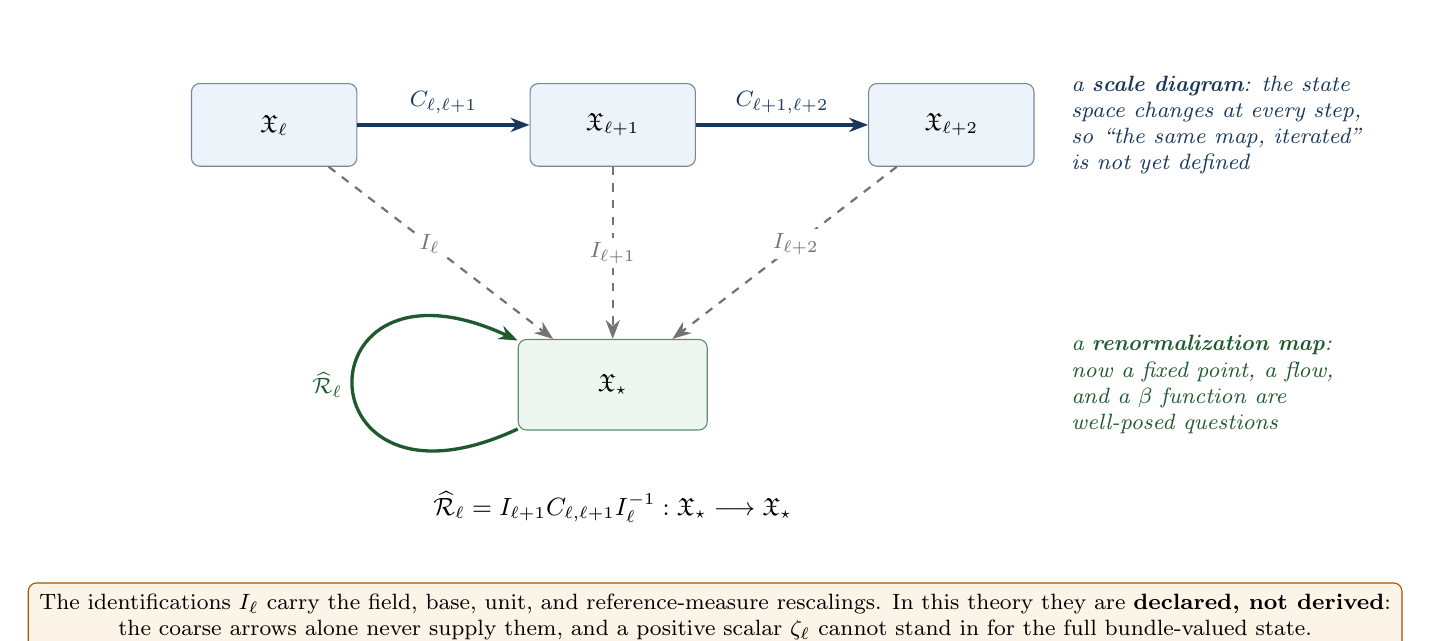
\begin{tikzpicture}[
  >={Stealth[length=2.4mm]},
  every node/.style={font=\small},
  sp/.style={draw=deepblue!60, fill=softblue, rounded corners=3pt,
             minimum width=2.1cm, minimum height=1.05cm, font=\small},
  ref/.style={draw=deepgreen!70, fill=softgreen, rounded corners=3pt,
              minimum width=2.4cm, minimum height=1.15cm, font=\small},
  ident/.style={->, dashed, thick, black!55}
]
\node[sp] (X0) at (0,3.5)  {$\mathfrak X_\ell$};
\node[sp] (X1) at (4.3,3.5) {$\mathfrak X_{\ell+1}$};
\node[sp] (X2) at (8.6,3.5) {$\mathfrak X_{\ell+2}$};
\draw[->, very thick, deepblue] (X0) -- node[above, font=\footnotesize]{$C_{\ell,\ell+1}$} (X1);
\draw[->, very thick, deepblue] (X1) -- node[above, font=\footnotesize]{$C_{\ell+1,\ell+2}$} (X2);
\node[anchor=west, font=\footnotesize\itshape, text=deepblue, align=left] at (10.0,3.5)
  {a \textbf{scale diagram}: the state\\ space changes at every step,\\
   so ``the same map, iterated''\\ is not yet defined};
\node[ref] (Xs) at (4.3,0.2) {$\mathfrak X_\star$};
\draw[ident] (X0) -- node[font=\footnotesize, fill=white, inner sep=1.5pt, pos=0.45]{$I_\ell$} (Xs);
\draw[ident] (X1) -- node[font=\footnotesize, fill=white, inner sep=1.5pt, pos=0.5]{$I_{\ell+1}$} (Xs);
\draw[ident] (X2) -- node[font=\footnotesize, fill=white, inner sep=1.5pt, pos=0.45]{$I_{\ell+2}$} (Xs);
\draw[->, very thick, deepgreen] (Xs) to[out=205,in=155,looseness=7]
  node[left, font=\footnotesize]{$\widehat{\mathcal R}_\ell$} (Xs);
\node[anchor=west, font=\footnotesize\itshape, text=deepgreen, align=left] at (10.0,0.2)
  {a \textbf{renormalization map}:\\ now a fixed point, a flow,\\
   and a $\beta$ function are\\ well-posed questions};
\node[font=\small] at (4.3,-1.35)
  {$\widehat{\mathcal R}_\ell=I_{\ell+1}C_{\ell,\ell+1}I_\ell^{-1}
    :\mathfrak X_\star\longrightarrow\mathfrak X_\star$};
\node[draw=orange!65!black, fill=softorange, rounded corners=3pt, align=center,
      font=\footnotesize, inner sep=4pt] at (5.6,-2.75)
  {The identifications $I_\ell$ carry the field, base, unit, and reference-measure rescalings.
   In this theory they are \textbf{declared, not derived}:\\
   the coarse arrows alone never supply them, and a positive scalar $\zeta_\ell$
   cannot stand in for the full bundle-valued state.};
\end{tikzpicture}}
\caption{\textbf{A scale diagram is not yet a renormalization group.} Coarse arrows between changing state spaces compose, but nothing is being iterated until declared isomorphisms identify every level with one reference object. Only then are fixed points, flows, and beta functions well posed.}
\label{fig:scale}
\end{figure}

Coarse arrows alone form a scale diagram: objects \(\mathfrak X_\ell\) indexed by resolution and morphisms composing consistently. They become a renormalization dynamics only after comparison data identify what is being compared across levels. Either levelwise re-embeddings or declared isomorphisms \(I_\ell:\mathfrak X_\ell\to\mathfrak X_\star\) must be supplied, and only the isomorphism option supplies the inverse needed to form
\begin{equation}
  \widehat{\mathcal R}_\ell=I_{\ell+1}C_{\ell,\ell+1}I_\ell^{-1}:\mathfrak X_\star\to\mathfrak X_\star.
  \label{eq:rg-map}
\end{equation}
Field, base, unit, and reference-measure rescalings are part of these maps. In this theory the state includes one principal bundle, two associated bundles, their possibly distinct connections, and both cross morphisms, and the manuscript records explicitly that a positive scalar normalization of one operator cannot stand for that state.

This is the honest version of a step physicists take without comment. After Kadanoff blocking one rescales lengths and fields to return to a comparable description, and the choice of that rescaling is what makes a fixed point meaningful. The manuscript declares the rescaling rather than deriving it, and says so.

\begin{boundarybox}
The finite exact scale theory supplies normalized kernels, pushed measure pairs, a bounded-action calculus with an exact conditional-variance loss, full Hoeffding interaction coordinates, and a typed projection residual. It supplies no thermodynamic limit. An infinite-volume limit still requires projectively consistent cylinder laws, boundary conditions or a DLR specification, tightness in a selected topology, convergence of free-energy densities, and compatible limits of the connection and cross-morphism components. A joint limit in system size and RG depth, together with basin independence and blocking-scheme robustness, is separately open, and a finite congruence identity or one matched exponent does not settle it.
\end{boundarybox}

\subsection{The identifications were then declared, and the composite measured}

On 2026-08-17 the finite categorical laboratory supplied the identifications of Figure~\ref{fig:scale} for a declared self-similar family, the nested-cycle tower, and measured the composite. Every threshold was fixed in the design before measurement, and each result below is a computation on declared finite instances, not a theorem beyond them.

The construction half behaved. The coarse link between adjacent parents is the Wilson line along the fine path joining their block roots, composed from the dressed boundary generators the mark-carrying parents already retain, and the holonomy of the coarse cycle equals the fine holonomy of the loop it encloses exactly, as group elements, with each block's interior holonomy retained as marks rather than discarded. Gauge covariance of the whole step holds to $10^{-12}$ on the coarse action, with one instructive condition: covariance forces the declared parent law to transform as data attached to the root frame. Feeding the blocking a frame-fixed prior breaks covariance by orders of magnitude, which is the variational analogue of forgetting that a background field must transform when the gauge does.

The composition law failed, decisively and informatively. Blocking six agents at once and blocking them in stages disagree by $0.204$ in sup norm on the final couplings against a pre-registered tolerance of $10^{-10}$, with a provably lossless intermediate projection, so the defect is the Bayes blocking kernel itself: the kernel family is not closed under composition across levels, for the same generic reason that lumped Markov chains are not Markov and compounded exponential families leave the family. The flow of Equation~\eqref{eq:rg-map} therefore exists per level pair but is a typed cocycle rather than an autonomous semigroup, and the composition defect is order one at every accessible depth and factorization, including two-then-three against three-then-two on an instance where both are legitimate.

What is fixed is fixed per ratio. For each declared blocking ratio the composite of blocking with the self-similar re-tiling is a measured local contraction on the reduced coupling space, spectral radius near $0.8$, and iterating it converges to a fixed structure whose pairwise block is zero to machine precision. That factorized subspace is provably invariant, because the block-local Bayes kernel sends factorized theories to factorized theories, and it is measured to be attracting, with pair-sector eigenvalues near $0.17$: in the level-local sense, interaction between parents is irrelevant, and all retained content settles into the single-site potential and the conserved connection. The ratio-two and ratio-three fixed structures differ by $0.81$ in relative sup norm, so even the endpoints of the flow are typed by the blocking ratio.

\begin{physicalreading}
Both the contraction and its triviality are the one-dimensional story a physicist already knows. The declared tower joins adjacent blocks through single boundary agents, so however large the blocks grow the interface stays one link wide, and a one-dimensional finite-range system with strictly positive weights has a Perron--Frobenius transfer matrix, exponentially decaying correlations, and no phase transition: block spins decouple under iteration exactly as in one-dimensional Ising decimation, where $\tanh K' = \tanh^2 K$ drives every finite coupling to zero. The instructive contrast is the hierarchical lattice of Berker--Ostlund and Migdal--Kadanoff, where each coarse bond aggregates a bundle of parallel fine paths and the bundle multiplicity sustains a genuine interacting fixed point. For a directed network of agents the question ``in what dimension does interaction survive'' therefore becomes ``which architectures renormalize to interacting fixed structures'': boundary multiplicity against per-link attenuation, an architecture property of the coupling graph rather than a property of any ambient space.
\end{physicalreading}

Two calibrations keep this result in proportion. Exact composability off a fixed point is not something standard real-space RG possesses either; it holds for pure decimation, asymptotically at fixed points, and on self-similar substrates built for it, and away from those cases renormalized interactions need not even exist. The claim the measurement refuted was stronger than standard lore warrants, and the laboratory caught that. And the measured fixed structures are consistent with the manuscript's own algebraic finding that its exhibited fixed sectors are trivial, now with a mechanism, a contraction rate, and a named architectural cause attached.

Everything above describes the \emph{passive} channel, in which the coarse coupling is inherited through blocking with attention frozen, and the follow-up measurements of 2026-08-17/18 changed the headline. Neither of the two structural rescues works for the passive channel: thickening the block boundary raises the one-step pair retention only sublinearly ($0.156$, $0.441$, $0.564$ at one, three, and six cut couplings per boundary) and saturates below one, and enlarging the parent alphabet with the smallest sector label, the block's belief-channel $Z_3$ charge in the singlet/triplet sense of Section~\ref{sec:trees-loops}, does not raise retention at all ($0.144$ against $0.156$, with the constant-sector control exact). What restores interaction is the theory's own re-binding rule: regenerating each level's attention from the flow-averaged transported divergence over the conserved connection and folding the alignment energy into the coarse action. Under that declared rule, itself gauge covariant to $10^{-11}$, the per-ratio composites converge to \emph{interacting} fixed structures — pairwise sup $0.579$ at ratio two and $0.625$ at ratio three, each about a quarter above its own one-step injection, with the maps still contracting. The physical moral is sharp: in this theory a tall hierarchy keeps its horizontal glue not by inheriting it but by actively re-establishing it at every level, using exactly the two ingredients blocking conserves, the connection and the coarse beliefs. The typed-cocycle verdict is unchanged by regeneration: composition defects stay order one ($0.17$--$0.27$) and the interacting fixed structures remain ratio-typed ($0.64$ relative sup), so which aggregation grain a hierarchy uses remains physically meaningful all the way to its endpoints.

\section{The Gaussian realization}

The multivariate Gaussian enters only after the general structure, as the tier in which every abstract object becomes an explicit matrix formula. It is a realization, not the definition of an agent, and the interaction subfamily consisting of a matrix-weighted Laplacian plus self terms is a declared subfamily rather than a consequence of every linear-Gaussian directed model.

Three results in this part are worth carrying away.

The first is that transported precision pooling is a theorem rather than a convention. For the anchored star model in which an apex latent \(b\) with proper prior \(\mathcal N(0,P_0^{-1})\) has conditionally independent constituents \(y_i\mid b\sim\mathcal N(\Theta_ib,R_i)\), the exact mean-field coordinate for the apex is Gaussian with precision
\begin{equation}
  P_b=P_0+\sum_{i=1}^n\Theta_i^\top R_i^{-1}\Theta_i,
  \label{eq:precision-addition}
\end{equation}
independent of the remaining factors. This is inverse-variance weighting with transports inserted, and it arises as an exact consequence of the joint rather than being posited. Read in the recognition direction it is a sufficiency statement: the statistic the constituents supply to the apex is \(\sum_i\Theta_i^\top R_i^{-1}y_i\), and Equation~\eqref{eq:precision-addition} is the precision that statistic carries.

The second is a convergence theorem. Under the exact block schedule that updates every constituent from the current apex and then updates the apex, the means obey an affine recursion with a unique fixed point, and in the norm induced by \(P_b\) the apex error contracts geometrically with rate
\begin{equation}
  \rho=\lambda_{\max}\bigl(P_b^{-1/2}BP_b^{-1/2}\bigr)<1,
  \qquad
  B=\sum_i\Theta_i^\top R_i^{-1}\Theta_i.
  \label{eq:contraction}
\end{equation}
The strict anchor \(P_0\succ0\) is essential; weakening it to positive semidefinite allows eigenvalue one and destroys both uniqueness and contraction. Delayed, noisy, asynchronous, and inexact updates are not covered and remain open.

The third is negative, and concerns closure under blocking. Unrestricted matrix-weighted Kron closure fails, and what survives is an exact closed congruence-diagonal domain with a qualified maximality boundary, together with a rectangular endpoint-map or cellular-sheaf category that is gauge covariant and closed under repeated linear-quadratic blocking. Compression of that richer cut datum to a single invertible graph link, with a normalized probability and rescaling lift retaining the global normalizer, is open.

On the flow itself the manuscript is deliberately narrow. Bi-additive Gaussian parameters are closed under additive pushforward, and an identified homogeneous hierarchy gives an operator fixed ray, but the ray lies on the boundary of the full-space Gaussian probability domain rather than in its interior. Attraction to it is a conjecture with named unproved ingredients, and infinite-hierarchy attraction, uniqueness within a basin, and blocking-scheme independence are open. Finite numerical gates test specified diagnostics; they do not prove asymptotic claims.

\section{The no-go: the tower needs a top}
\label{sec:nogo}

The most physically interesting negative result in the manuscript concerns an ambition it then refutes in a precisely bounded way. A tower of scales in which every level's prior is supplied by the level above must terminate, and the natural way to avoid a declared top is to close the tower with a reciprocal pair: two latents, each supplying a penalty for the other.

Consider two latents \(u,v\in\mathbb R^K\) joined by distinct parallel edge copies with link transports \(\Theta_e\) and \(\Theta_f\), assembling the precision
\begin{equation}
  J=E_e^\top R_e^{-1}E_e+E_f^\top R_f^{-1}E_f,
  \qquad
  E_e=\begin{pmatrix}I&-\Theta_e\end{pmatrix},
  \quad
  E_f=\begin{pmatrix}-\Theta_f&I\end{pmatrix},
  \label{eq:pair-precision}
\end{equation}
and write \(H=\Theta_f\Theta_e\) for the holonomy of the two-cycle. The kernel is computed exactly and does not depend on the link covariances at all:
\begin{equation}
  \ker J=\bigl\{(\Theta_ev,v):v\in\ker(H-I)\bigr\},
  \qquad
  \dim\ker J=\dim\ker(H-I).
  \label{eq:pair-kernel}
\end{equation}
The determinant is equally clean,
\begin{equation}
  \det J=\frac{\bigl(\det(I-H)\bigr)^2}{\det R_e\det R_f},
  \label{eq:det-holonomy}
\end{equation}
so the link data enter only through the holonomy of the loop.

If the two edge copies give the same flat endpoint comparison, so that \(\Theta_f=\Theta_e^{-1}\) and \(H=I\), the kernel is all of \(\mathbb R^K\) and the assembled precision is singular for every choice of positive definite link covariances. The flat direction consists precisely of the transport-consistent configurations, those in which the two latents agree after transport. The unanchored flat pair charges exactly nothing there, so it supplies no coercivity along the very direction it was introduced to control, and there is no normalized Lebesgue density for the variational identity to apply to.

\begin{physicalreading}
This is a zero mode of a pure-gauge configuration, and Equation~\eqref{eq:det-holonomy} says the spectrum of the obstruction depends on the link variables only through the Wilson loop. The zero mode is lifted exactly when the holonomy has no fixed vector. The Aharonov--Bohm situation is the same structure: a particle on a ring has a degeneracy that depends only on the enclosed flux, and threading nontrivial flux splits it. Here nontrivial holonomy makes the assembled precision positive definite, and the set of holonomies at which it fails is the zero locus of \(\det(H-I)\), a proper algebraic subset with dense complement.
\end{physicalreading}

The boundary of this no-go is drawn carefully, and a reader should not take away more than it says. It is not a theorem against cycles. Adding a proper anchor at each vertex makes the total precision positive definite, and the resulting globally normalized Gaussian Markov random field is a legitimate probability model with a finite partition function; what is lost is the convenience of a product of locally normalized directed kernels, not existence. What the anchored model does not restore is the ability to treat the normalization as a constant, since the transports enter the log determinant and the manuscript exhibits an explicit witness in which that dependence is nonconstant. An objective that appends the reciprocal energy while omitting the global normalizer is not an evidence bound at all.

There is also a structural reason the ambition could not have succeeded. In any finite directed acyclic generative model there is at least one latent with no parents, whose marginal law is therefore part of the declared parameters. No finite acyclic construction can have every prior constituted by other latents, so the failure is not for want of ingenuity. Replacing a declared prior by a declared edge link relocates the declaration rather than removing it.

What survives is the anchored star of Equation~\eqref{eq:precision-addition}, and with it the participatory content that motivated the fold in the first place. At a variational fixed point the apex belief is a transported pooling of every constituent's current belief, and each constituent's effective prior in its own update is that apex belief transported back down. Each agent's input is constituted by the apex update and the apex input is constituted by the agents' updates. This is a loop in an inference algorithm, not a cycle in the factorization of the model: every step is a coordinate update of a trial law against a joint that remains fixed, acyclic, and normalized, so nothing reads a posterior into a generative kernel.

\begin{translationbox}
The bidirectional dependence that a participatory reading wants is available, and it lives in the solver rather than in the model. That is a weaker claim than the one the fold was reaching for, and the manuscript says so rather than blurring the two.
\end{translationbox}

\section{What is proved, what is declared, and what is open}

The manuscript tags every nontrivial statement with one of seven statuses, and the taxonomy is worth reproducing because it is the most transferable thing in the document. \textsc{established} means proved here or cited to a checked source. \textsc{definition} means a declared type or convention, with nothing being proved. \textsc{hypothesis} means a restriction adopted by choice, with its exclusions stated. \textsc{conjecture} means believed, precisely stated, and unproved. \textsc{numerical} means supported by computation only. \textsc{open} means unsettled, with what would settle it named. \textsc{not-claimed} means a statement the development deliberately declines to make, which is not the same as refuting it.

\begin{table}[ht]
\centering
\small
\begin{tabularx}{\textwidth}{>{\raggedright\arraybackslash}p{0.16\textwidth}X}
\toprule
\textbf{Status} & \textbf{Content} \\
\midrule
Established &
The typed bundle and kernel contract; the exact evidence identity and its extended-real form, with the equality criterion and the insufficiency of marginal matching; the total-correlation chain identity; the exact local--global potential identity for arbitrary blocks; the attention-label posterior, canonical row free energy, and replicator flow under declared hypotheses; passive gauge covariance of the Fisher and Amari pullbacks with exact connection-change formulas; extended data processing with its equality condition; the evidence-preserving coarse channel and the exact coarse free-energy identity with its nonnegative defect; the full pointwise parent datum; exact finite-network interaction coordinates and the Hoeffding action isomorphism; congruence-diagonal Kron closure with qualified maximality; frame invariance of the generalized spectrum; the reciprocal-pair kernel and determinant identities; the anchored-star definiteness, precision-addition, and geometric contraction theorems; and typed-intervention nonidentifiability in its declared categories. \\
\addlinespace
Hypothesis &
The selected smooth tier for differential statements; regular observations selecting a posterior version; absolute continuity of the recognition law; label exclusivity and row factorization for the attention softmax; the Laplacian-plus-self-term interaction cone; identification of graph links with base transports; the Fisher metric as the declared fiber geometry; and observational closure as the sole interpretive restriction. \\
\addlinespace
Numerical &
Deterministic replacement checks for the generalized spectrum, the star and flat-pair contrast, and the holonomy determinant and kernel dimensions; the 2026-08-17 rescaling-map measurements on the nested-cycle family: exact gauge covariance and holonomy conservation of the declared step, the refuted compatibility law (composition defect $0.204$ against a pre-registered $10^{-10}$), and contracting per-ratio composites whose passive fixed structures are factorized and ratio-typed; and the 2026-08-17/18 follow-ups: sublinear boundary-multiplicity retention, the null sector-capacity result, and the regenerated-attention composites converging to interacting, still ratio-typed fixed structures. These establish usability under their declared protocols and are not proofs. \\
\addlinespace
Open &
The continuum law theory and the thermodynamic limit; joint limits in system size and RG depth, with universality, basin independence, and blocking-scheme robustness; a canonical channel, membership, and partition selector; grand-canonical edge or membership occupation; recursive networks of parent probabilistic data; participatory cross-scale feedback and sustained nonequilibrium; the comparison-category theorem and category-independent intervention semantics; a smooth scale tier and a canonical continuous beta function; multiplicative ergodic structure of the interaction cocycle; nonflat-link compression; convergence of the alternating scheme and robustness to delayed or asynchronous updates; a global relational information clock; an operational observable sensitive to base holonomy; a canonical connection and a nondegenerate pullback geometry; which boundary-multiplicity architectures of the coupling graph sustain interacting fixed structures; whether the measured composition defect contracts on deeper flows or persists; and identification of any limiting object with a physical law. \\
\addlinespace
Not claimed &
That \(\mathcal C\) is physical spacetime, or carries a Lorentzian signature, causal cones, a measure, or a field equation; that Fisher duration is physical time, proper time, thermal time, or a quantum clock; that RG depth is inference time; that graph-link holonomy evidences base curvature or bundle topology; that autonomous agency emerges; and that any structural-realist reading follows from the invariance results. \\
\bottomrule
\end{tabularx}
\caption{The boundary of the theory, compressed. Each row is a summary of many individually tagged statements; the manuscript's own ledger appendix is authoritative.}
\label{tab:status}
\end{table}

\begin{provedbox}
The load-bearing achievements are a consistent typed gauge-covariant kinematics for probabilistic agents, one exact variational identity that survives it, an exact potential identity making local multi-agent updates coordinate descent on one collective free energy, a canonical source-selection ensemble with a correctly normalized row free energy, an exact accounting of the information destroyed by any normalized coarse channel, a full static pointwise parent probabilistic datum, and a set of sharp finite counterexamples that fence off invalid shortcuts.
\end{provedbox}

\begin{boundarybox}
What is not achieved is equally definite. There is no continuum limit, no thermodynamic limit, no derived rescaling, no canonical connection, no proved nontrivial fixed point with a basin, no derivation of agency, and no identification of anything in the formalism with a physical law, a physical clock, or a spacetime. The finite static theorems are not empirically inconclusive; they are mathematical statements. What remains empirically inconclusive is their proposed physical and cross-scale interpretation. Any viable interpretation must continue to distinguish graph-link holonomy, base-connection holonomy, bundle topology, and gauge redundancy, and must state which of them its evidence bears on.
\end{boundarybox}

\section{What a physicist should take away}

Four things in this program are worth a physicist's attention, and one temptation is worth resisting.

The first is that the gauge structure is not decorative. Agents holding probabilistic beliefs in local frames genuinely have a comparison problem, transport genuinely resolves it, and loop transport genuinely fails to be trivial. The lattice analogy is exact at the level of the link variables and their Wilson loops, and the trivializing criterion is literally the pure-gauge criterion. Where the analogy stops is that the matter fields are probability laws, so the group acts by pushforward and the fibers carry no linear structure; a good deal of the manuscript's length is the price of that one substitution.

The second is the exact information accounting. Equation~\eqref{eq:coarse-vfe} is a clean statement about what blocking costs, valid without Gaussian assumptions, without a mean-field restriction, and in the extended reals so that it survives singular trial laws. A physicist used to controlling truncation error heuristically may find it worth having a quantity that is exactly the discarded information rather than a bound on it.

The third is the thermodynamic hierarchy. Variational free energy has an exact expected-energy minus entropy decomposition in natural units, and each attention row is a canonical ensemble over possible sources. The temperature is \(\tau_i\), while \(\beta_{ij}\) is a normalized occupation probability. Writing \(\beta_{ij}D_{ij}=-\mu_{ij}N_{ij}\) is only an algebraic resemblance to a grand potential because the normalized row has no fluctuating count. A genuine grand-canonical network requires explicit occupation variables, a count, and chemical potentials conjugate to that count. That extension is natural, but it is not yet part of the established theory.

The fourth is the discipline about status. The manuscript refuses to let a suggestive correspondence stand as a theorem, and its most useful sections are the ones that say what would be required to close a gap. The list of things that would make the interpretation testable, including a preregistered target system, at least two admissible partitions, declared blocking and rescaling maps, gauge alignment, a held-out statistic, an acceptance tolerance, and Gaussian-graphical and spectral baselines, is an experimental protocol sketch rather than a gesture.

The temptation to resist is reading the base as spacetime. The word ``holonomy'' and the presence of a principal bundle invite it, and the manuscript blocks it repeatedly and deliberately. Nothing in the construction supplies a signature, a causal structure, a measure on the base, or an equation of motion for it, and the pullback tensors that do live on the base are relative to a connection that is never canonically chosen. Whether any of this can be connected to physics is the open question the program names as its own, and it has not been answered.

\section{Where to read further}

The manuscript's own fast path for a physicist is worth following. Take the object and frame-covariance contract from the introduction and the geometry chapter, then read only the normalized-joint and evidence identities in the probability, generative, and ELBO chapters. On a second pass read the local--collective potential theorem and the attention construction, then the covariant pullback and relational-history chapters. On a third pass take the three-operation distinction, the Markov coarse theorem, the exact network closure, and the typed scale diagram. The Gaussian spine is then the interaction cone, the recognition costs and Fisher geometry, and finally Gaussian aggregation, Kron closure, holonomy, fixed rays, and the numerical gates. The obstruction and interpretation chapters separate the exact negative results from the empirical and interpretive commitments, and the claim ledger collects every open obligation in one place.

For the static coarse-graining theorem specifically, the companion guide \path{solid_RG_theory.tex} treats the same material at a level between this document and the manuscript, with the measure-theoretic steps written out. The proposed thermodynamic extension is developed in \path{Theory/grand_canonical_meta_agent_formation.tex}; it should be read as a research program built on the established attention and parent-construction theorems, not as another chapter of proved results.

\begin{thebibliography}{9}

\bibitem{Friston2010}
K.~Friston,
``The free-energy principle: a unified brain theory?,''
\emph{Nature Reviews Neuroscience} \textbf{11}, 127--138 (2010),
\href{https://doi.org/10.1038/nrn2787}{doi:10.1038/nrn2787}.

\bibitem{Jaynes1957}
E.~T.~Jaynes,
``Information theory and statistical mechanics,''
\emph{Physical Review} \textbf{106}, 620--630 (1957),
\href{https://doi.org/10.1103/PhysRev.106.620}{doi:10.1103/PhysRev.106.620}.

\bibitem{ParkNewman2004}
J.~Park and M.~E.~J.~Newman,
``Statistical mechanics of networks,''
\emph{Physical Review E} \textbf{70}, 066117 (2004),
\href{https://doi.org/10.1103/PhysRevE.70.066117}{doi:10.1103/PhysRevE.70.066117}.

\bibitem{GrossBlasius2008}
T.~Gross and B.~Blasius,
``Adaptive coevolutionary networks: a review,''
\emph{Journal of the Royal Society Interface} \textbf{5}, 259--271 (2008),
\href{https://doi.org/10.1098/rsif.2007.1229}{doi:10.1098/rsif.2007.1229}.

\bibitem{Wilson1974}
K.~G.~Wilson,
``Confinement of quarks,''
\emph{Physical Review D} \textbf{10}, 2445--2459 (1974),
\href{https://doi.org/10.1103/PhysRevD.10.2445}{doi:10.1103/PhysRevD.10.2445}.

\bibitem{Kogut1979}
J.~B.~Kogut,
``An introduction to lattice gauge theory and spin systems,''
\emph{Reviews of Modern Physics} \textbf{51}, 659--713 (1979),
\href{https://doi.org/10.1103/RevModPhys.51.659}{doi:10.1103/RevModPhys.51.659}.

\end{thebibliography}

\end{document}
